%%%%%%%%%%%%%%%%%%%%%%%%%%%%%%%%%%%%%%%%%%%%%%%%%%%%%%%%%%%%%%%%%%%%%%
% Overleaf (WriteLaTeX) Example: Molecular Chemistry Presentation
%
% Source: http://www.overleaf.com
%
% In these slides we show how Overleaf can be used with standard 
% chemistry packages to easily create professional presentations.
% 
% Feel free to distribute this example, but please keep the referral
% to overleaf.com
% 
%%%%%%%%%%%%%%%%%%%%%%%%%%%%%%%%%%%%%%%%%%%%%%%%%%%%%%%%%%%%%%%%%%%%%%

\documentclass{beamer}

\mode<presentation>
{
  \usetheme{Madrid}       % or try default, Darmstadt, Warsaw, ...
  \usecolortheme{default} % or try albatross, beaver, crane, ...
  \usefonttheme{default}    % or try default, structurebold, ...
  \setbeamertemplate{navigation symbols}{}
  \setbeamertemplate{caption}[numbered]
} 

\usepackage[english]{babel}
\usepackage[utf8x]{inputenc}
\usepackage{chemfig}
\usepackage[version=3]{mhchem}

\usepackage{hyperref}
  \hypersetup{colorlinks=true}
  \hypersetup{urlcolor=blue}
  \hypersetup{linkcolor = .}
\usepackage{xcolor}
\usepackage{siunitx}
  \sisetup{separate-uncertainty = true}
\usepackage{physics}
\usepackage[font=small,labelfont=bf]{caption}
\usepackage{subcaption}
\usepackage[en-GB]{datetime2}
\usepackage{feynmp}
\DeclareGraphicsRule{*}{mps}{*}{}

\usepackage{scalerel}
\newcommand{\mylbrace}[2]{\vspace{#2pt}\hspace{6pt}\scaleleftright[\dimexpr5pt+#1\dimexpr0.06pt]{\lbrace}{\rule[\dimexpr2pt-#1\dimexpr0.5pt]{-4pt}{#1pt}}{.}}
\newcommand{\myrbrace}[2]{\vspace{#2pt}\scaleleftright[\dimexpr5pt+#1\dimexpr0.06pt]{.}{\rule[\dimexpr2pt-#1\dimexpr0.5pt]{-4pt}{#1pt}}{\rbrace}\hspace{6pt}}

% Here's where the presentation starts, with the info for the title slide
\title[$B^\pm\to(K^+K^-\pi^+\pi^-)_DK^\pm$]{Measuring \texorpdfstring{$\gamma$}{gamma} in \texorpdfstring{$B^\pm\to(K^+K^-\pi^+\pi^-)_DK^\pm$}{B to K+K-pi+pi-} decays}
\author{Martin Tat}
\institute{Oxford LHCb}
\date{\today}

\titlegraphic{
\includegraphics[width = 4cm]{lhcb.jpg}\hspace{3cm}~%
              \reflectbox{
\includegraphics[width = 4cm]{lhcb.jpg}}}

\begin{document}

\begin{frame}
  \titlepage
\end{frame}

% These three lines create an automatically generated table of contents.
\begin{frame}{Outline}
  \tableofcontents
\end{frame}

\section{Background}
\begin{frame}{Background}
  \begin{itemize}
    \item Supervisors:
    \begin{itemize}
      \item{Prof Guy Wilkinson ($\gamma$ measurement)}
      \item{Prof Neville Harnew (TORCH)}
    \end{itemize}
    \item 4-year MPhys in Oxford
    \begin{itemize}
      \item Performance of monolithic CMOS sensors
      \item Prof Daniela Bortoletto
    \end{itemize}
    \item CERN Summer Student 2019
    \begin{itemize}
      \item Beam loss reduction in TT$20$ transfer line
      \item Dr Yann Dutheil, Dr Matthew Fraser
    \end{itemize}
    \item Oxford Summer Student 2018
    \begin{itemize}
      \item Study of PDF uncertainties in W-boson mass measurement
      \item Prof Chris Hays
    \end{itemize}
    \item RAL Summer Student 2018
    \begin{itemize}
      \item Bending magnets in accelerator simulations
      \item Dr Chris Rogers
    \end{itemize}
  \end{itemize}
\end{frame}

\section{\texorpdfstring{$\gamma$}{gamma} and the unitary triangle}
\begin{frame}{$\gamma$ and the unitary triangle}
  \begin{center}
    Unitarity of CKM matrix: $V_{ud}V^*_{ub} + V_{cd}V^*_{cb} + V_{td}V^*_{tb} = 0$ \\
    \vspace{0.4cm}
    Define $\gamma = \text{arg}\Big(-\frac{V_{ud}V^*_{ub}}{V_{cd}V^*_{cb}}\Big)$
  \end{center}
  \vspace{-0.2cm}
  \begin{figure}
    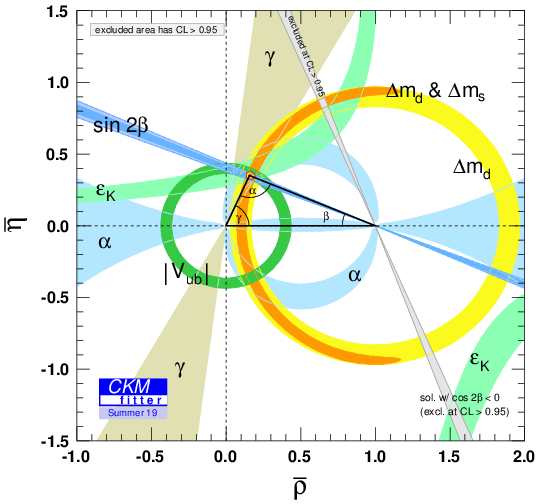
\includegraphics[scale = 0.3]{ckmfitter.png}
  \end{figure}
  \vspace{-0.4cm}
  \begin{center}
    CKMfitter Group (J. Charles et al.), Eur. Phys. J. C41, 1-131 (2005)
  \end{center}
\end{frame}

\begin{frame}{\texorpdfstring{$\text{b}\to\text{u}$}{b to u} and \texorpdfstring{$\text{b}\to\text{c}$}{b to c} interference}
  \begin{figure}[H]
    \centering
    \vspace{0.3cm}
    \begin{subfigure}{0.5\textwidth}
      \centering
      \begin{fmffile}{fgraph_BtoDK1}
        \setlength{\unitlength}{0.4cm}
        \begin{fmfgraph*}(6,6)
          \fmfstraight
          \fmfleft{i1,B,i2,t1,t2,t3,t9,t10}
          \fmfright{o1,D,o2,t4,t5,o3,K,o4}
          \fmflabel{$\bar{u}$}{i1}
          \fmflabel{$b$}{i2}
          \fmfv{l.d=20,l.a=180,l={$B^-$\mylbrace{30}{-8}}}{B}
          \fmflabel{$\bar{u}$}{o1}
          \fmflabel{$c$}{o2}
          \fmflabel{$\bar{u}$}{o3}
          \fmflabel{$s$}{o4}
          \fmfv{l.d=15,l.a=0,l={\myrbrace{30}{-12}}$D^0$}{D}
          \fmfv{l.d=15,l.a=0,l={\myrbrace{30}{11}}$K^-$}{K}
          \fmf{fermion}{o1,i1}
          \fmf{fermion,tension=1.5}{i2,v1}
          \fmf{fermion}{v1,o2}
          \fmf{phantom,tension=1.5}{t9,v2}
          \fmf{boson,label=$W$,label.side=left,tension=0}{v1,v2}
          \fmf{fermion}{v2,o4}
          \fmf{fermion}{o3,v2}
        \end{fmfgraph*}
      \end{fmffile}
      \vspace{0.5cm}
      \caption{$B^-\to D^0K^-$}
    \end{subfigure}%
    \begin{subfigure}{0.5\textwidth}
      \centering
      \begin{fmffile}{fgraph_BtoDK2}
        \setlength{\unitlength}{0.4cm}
        \begin{fmfgraph*}(6,6)
          \fmfstraight
          \fmfleft{i1,t1,t2,B,t9,t10,i2}
          \fmfright{o1,K,o2,t4,t5,o3,D,o4}
          \fmflabel{$\bar{u}$}{i1}
          \fmflabel{$b$}{i2}
          \fmfv{l.d=20,l.a=180,l={$B^-$\mylbrace{100}{-8}}}{B}
          \fmflabel{$\bar{u}$}{o1}
          \fmflabel{$s$}{o2}
          \fmflabel{$\bar{c}$}{o3}
          \fmflabel{$u$}{o4}
          \fmfv{l.d=15,l.a=0,l={\myrbrace{30}{13}}$\bar{D^0}$}{D}
          \fmfv{l.d=15,l.a=0,l={\myrbrace{30}{-13}}$K^-$}{K}
          \fmf{fermion}{o1,i1}
          \fmf{fermion,tension=1.5}{i2,v1}
          \fmf{fermion}{v1,o4}
          \fmf{phantom,tension=1.5}{t2,v2}
          \fmf{boson,label=$W$,label.side=left,tension=0}{v1,v2}
          \fmf{fermion}{v2,o2}
          \fmf{fermion}{o3,v2}
        \end{fmfgraph*}
      \end{fmffile}
      \vspace{0.5cm}
      \caption{$B^-\to\bar{D^0}K^-$}
    \end{subfigure}
  \end{figure}
  \vspace{0.3cm}
  \begin{center}
    Similar diagrams for $B^+\to DK^+$, with $\gamma\to -\gamma \implies$ \\
    \vspace{0.3cm}
    Inteference when $D^0$ and $\bar{D^0}$ decay into a common final state\\
    \vspace{0.3cm}
    Single most precise measurement: $\gamma = (68.7^{+5.2}_{-5.1})^\circ$ \href{https://arxiv.org/abs/2010.08483}{arXiv:2010.08483} \\
    $B^\pm\to DK^\pm$, $B^\pm\to D\pi^\pm$, $D\to K_S^0h^+h^-$
  \end{center}
\end{frame}

\section{The \texorpdfstring{$D\to K^+K^-\pi^+\pi^-$}{D to K+K-pi+pi-} decay}
\begin{frame}{The $D\to K^+K^-\pi^+\pi^-$ decay}
  \begin{itemize}
    \item{Estimated $2000$ events from LHCb Run $1$ and $2$}
    \vspace{0.2cm}
    \item{First proposed by G. Wilkinson and J. Rademacker \href{https://arxiv.org/abs/hep-ph/0611272}{arXiv:hep-ph/0611272}}
    \begin{itemize}
      \item{Amplitude analysis: Isobar model}
      \item{Estimated $\gamma$ precision: $\SI{14}{\degree}$ with $1000$ events}
    \end{itemize}
    \vspace{0.2cm}
    \item{CLEO amplitude analysis \href{https://arxiv.org/abs/1201.5716}{arXiv:1201.5716}}
    \begin{itemize}
      \item{Estimated $\gamma$ precision: $\SI{11}{\degree}$ with $2000$ events}
    \end{itemize}
    \vspace{0.2cm}
    \item{LHCb amplitude analysis \href{https://arxiv.org/abs/1811.08304}{arXiv:1811.08304}}
    \begin{itemize}
      \item{AmpGen for generating events and unbinned fit}
    \end{itemize}
    \vspace{0.2cm}
    \item{Other $4$-body decay studies:}
    \begin{itemize}
      \item{Binned analysis of $K_S^0\pi^+\pi^-\pi^0$ by Belle \href{https://arxiv.org/abs/1908.09499}{arXiv:1908.09499}}
      \item{Inclusive analysis of $h^\pm\pi^\mp\pi^+\pi^-$ \href{https://arxiv.org/abs/1906.08297}{arXiv:1906.08297}, \href{https://arxiv.org/abs/1709.05855}{arXiv:1709.05855}, \href{https://arxiv.org/abs/1603.08993}{arXiv:1603.08993} by LHCb}
    \end{itemize}
  \end{itemize}
\end{frame}

\begin{frame}{Unbinned fit with amplitude model}
  \vspace{-0.3cm}
  \begin{align*}
    \mathcal{A}(B^-\to(K^+K^-\pi^+\pi^-)_DK^-) =& \mathcal{A}_B\mathcal{A}(D^0\to K^+K^-\pi^+\pi^-) \\
  +& \mathcal{A}_B\mathcal{A}(\bar{D^0}\to K^+K^-\pi^+\pi^-)r_Be^{i(\delta_B - \gamma)}
  \end{align*}
  \vspace{-0.5cm}
  \begin{itemize}
    \item{$\mathcal{A}(D\to K^+K^-\pi^+\pi^-)$ obtained from amplitude model}
    \item{Fit with $\gamma$, $\delta_B$ and $r_B$ as free parameters}
    \item{Initial values:}
    \begin{itemize}
      \item{$\gamma = \SI{75}{\degree}$}
      \item{$\delta_B = \SI{130}{\degree}$}
      \item{$r_B = \SI{0.1}{}$}
    \end{itemize}
    \item{Results from unbinned fit of $\SI{2e3}{}$ events:}
    \begin{itemize}
      \item{$\gamma = \SI{69(11)}{\degree}$}
      \item{$\delta_B = \SI{115(11)}{\degree}$}
      \item{$r_B = \SI{0.098(17)}{}$}
    \end{itemize}
    \item{Results from unbinned fit of $\SI{2e4}{}$ events:}
    \begin{itemize}
      \item{$\gamma = \SI{77.1(35)}{\degree}$}
      \item{$\delta_B = \SI{129(4)}{\degree}$}
      \item{$r_B = \SI{0.093(6)}{}$}
    \end{itemize}
  \end{itemize}
\end{frame}

\section{Unbinned fit with amplitude model}
\begin{frame}{Unbinned fit of $\SI{2e3}{}$ events with amplitude model}
  \begin{figure}
    \centering
    \vspace{-0.2cm}
    \begin{subfigure}{0.46\textwidth}
      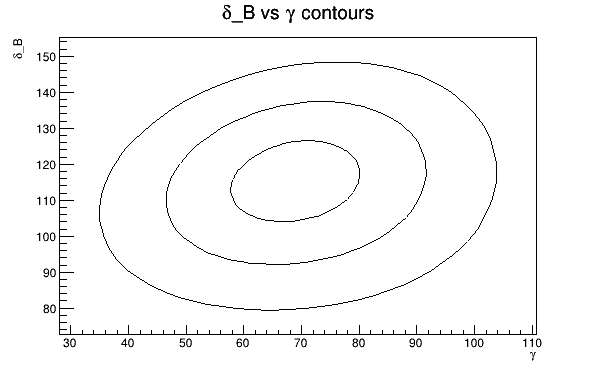
\includegraphics[width = 1.0\textwidth]{Contour_dB_vs_gamma_1K.png}
      \caption{$\gamma$ vs $\delta_B$}
    \end{subfigure}%
    \begin{subfigure}{0.46\textwidth}
      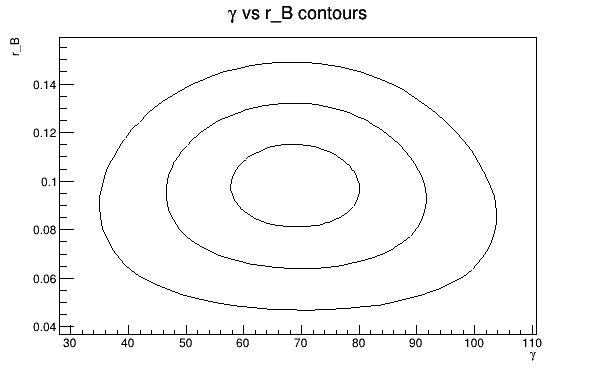
\includegraphics[width = 1.0\textwidth]{Contour_gamma_vs_rB_1K.png}
      \caption{$\gamma$ vs $r_B$}
    \end{subfigure}
    \begin{subfigure}{0.46\textwidth}
      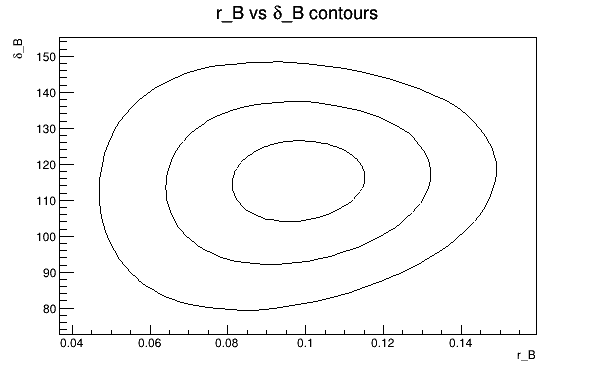
\includegraphics[width = 1.0\textwidth]{Contour_rB_vs_dB_1K.png}
      \caption{$r_B$ vs $\delta_B$}
    \end{subfigure}
  \end{figure}
\end{frame}

\begin{frame}{Unbinned fit of $\SI{2e4}{}$ events with amplitude model}
  \begin{figure}
    \centering
    \vspace{-0.2cm}
    \begin{subfigure}{0.46\textwidth}
      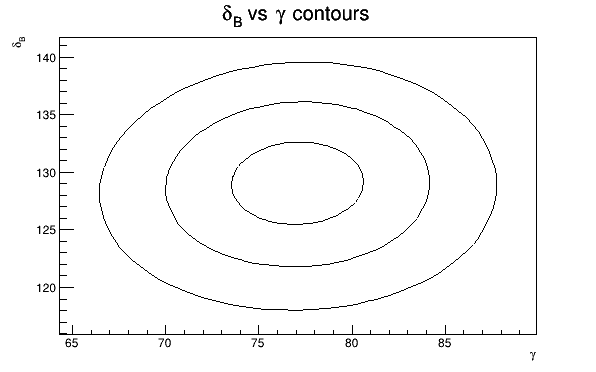
\includegraphics[width = 1.0\textwidth]{Contour_dB_vs_gamma_10K.png}
      \caption{$\gamma$ vs $\delta_B$}
    \end{subfigure}%
    \begin{subfigure}{0.46\textwidth}
      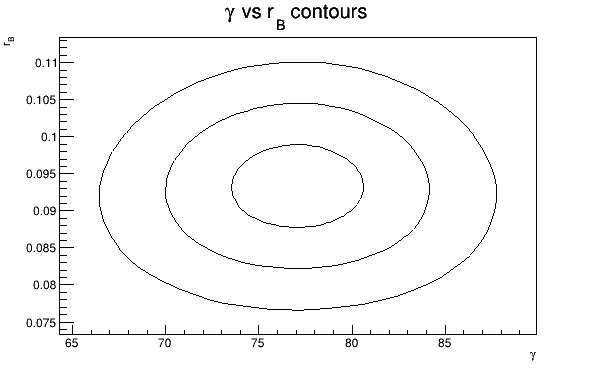
\includegraphics[width = 1.0\textwidth]{Contour_gamma_vs_rB_10K.png}
      \caption{$\gamma$ vs $r_B$}
    \end{subfigure}
    \begin{subfigure}{0.46\textwidth}
      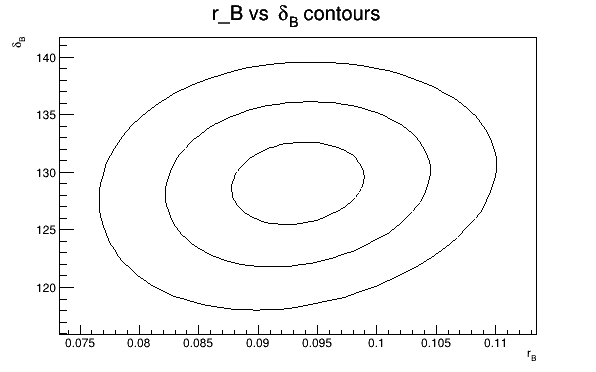
\includegraphics[width = 1.0\textwidth]{Contour_rB_vs_dB_10K.png}
      \caption{$r_B$ vs $\delta_B$}
    \end{subfigure}
  \end{figure}
\end{frame}

\section{Binned fit of \texorpdfstring{$D\to K^+K^-\pi^+\pi^-$}{D to K+K-pi+pi-}}
\begin{frame}{Binned fit of $D\to K^+K^-\pi^+\pi^-$}
  \vspace{-0.5cm}
  \begin{align*}
    \mathcal{A}(B^-\to(K^+K^-\pi^+\pi^-)_DK^-) =& \mathcal{A}_B\mathcal{A}(D^0\to K^+K^-\pi^+\pi^-) \\
  +& \mathcal{A}_B\mathcal{A}(\bar{D^0}\to K^+K^-\pi^+\pi^-)r_Be^{i(\delta_B - \gamma)}
  \end{align*}
  \vspace{-0.5cm}
  \begin{block}{Event yield in bin $i$}
    $N^-_i = h_{B^-}\Big(K_i + \big(x_-^2 + y_-^2\big)\bar{K_i} + 2\sqrt{K_i\bar{K_i}}\big(x_-c_i + y_-s_i\big)\Big)$
    $N^+_i = h_{B^+}\Big(\bar{K_i} + \big(x_+^2 + y_+^2\big)K_i + 2\sqrt{K_i\bar{K_i}}\big(x_+c_i - y_+s_i\big)\Big)$
  \end{block}
  \begin{block}{CP-violating observables}
    $x_\pm = r_B\cos(\delta_B\pm\gamma), \quad y_\pm = r_B\sin(\delta_B\pm\gamma)$
  \end{block}
  \begin{itemize}
    \item{$c_i$, $s_i$: Amplitude-averaged strong phase difference of $D$ decay}
    \item{Measure $c_i$ and $s_i$ at BES III detector}
    \item{Can measure $K_i$ and $\bar{K_i}$ at both LHCb and BES III}
    \item{Need to divide phase space into bins}
  \end{itemize}
\end{frame}

\begin{frame}{Pull study with $\SI{2e3}{}$ events}
  \begin{figure}
    \centering
    \vspace{-0.2cm}
    \begin{subfigure}{0.5\textwidth}
      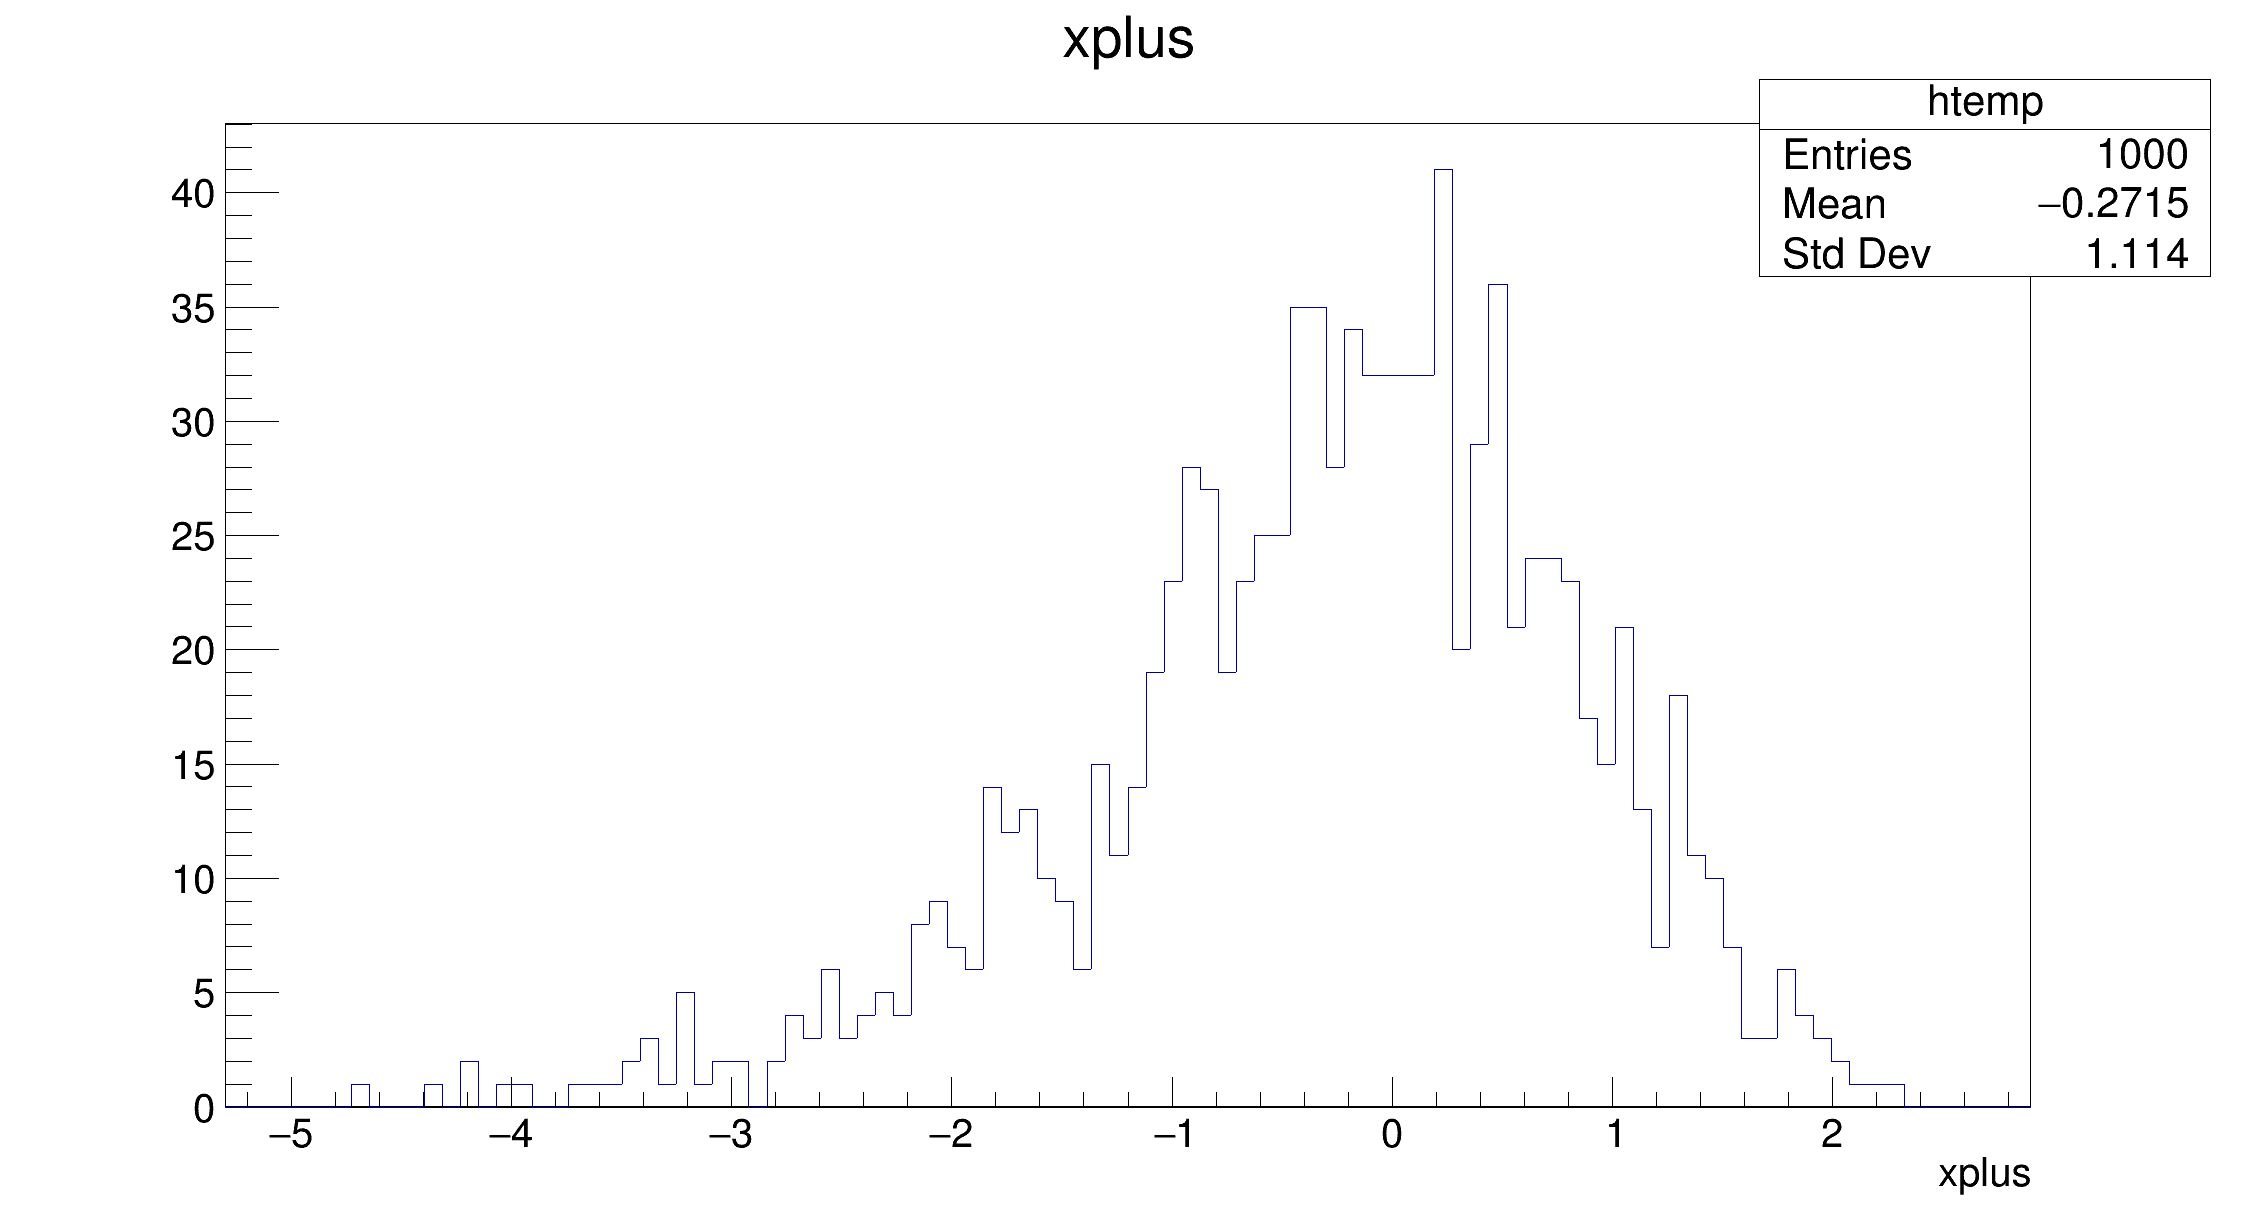
\includegraphics[width = 1.0\textwidth]{xplus1K1K.png}
      \caption{$x_+$ pull}
    \end{subfigure}%
    \begin{subfigure}{0.5\textwidth}
      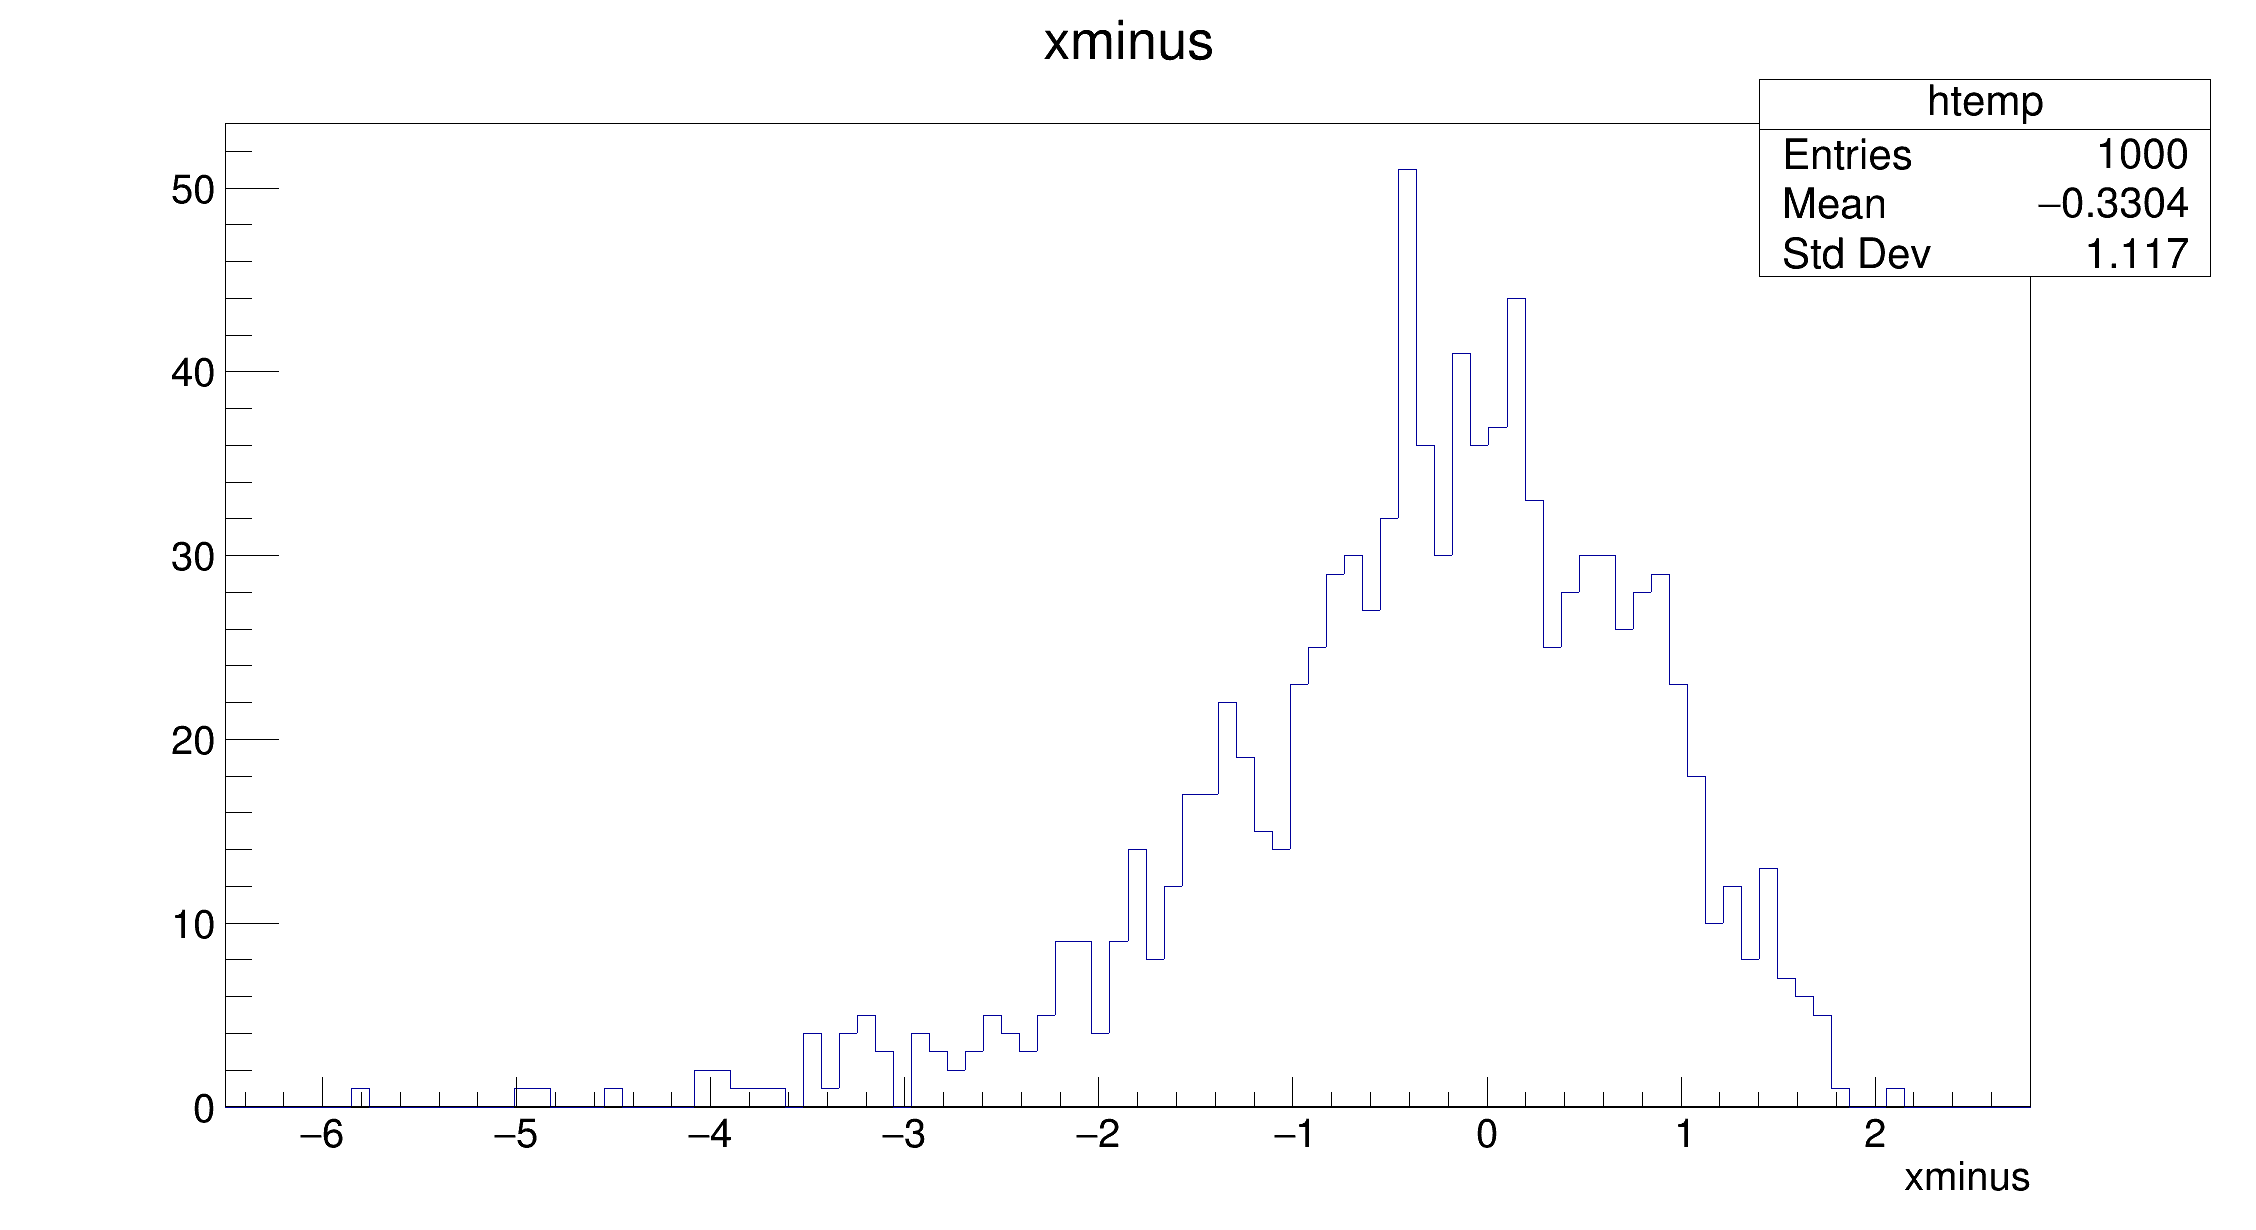
\includegraphics[width = 1.0\textwidth]{xminus1K1K.png}
      \caption{$x_-$ pull}
    \end{subfigure}
    \begin{subfigure}{0.5\textwidth}
      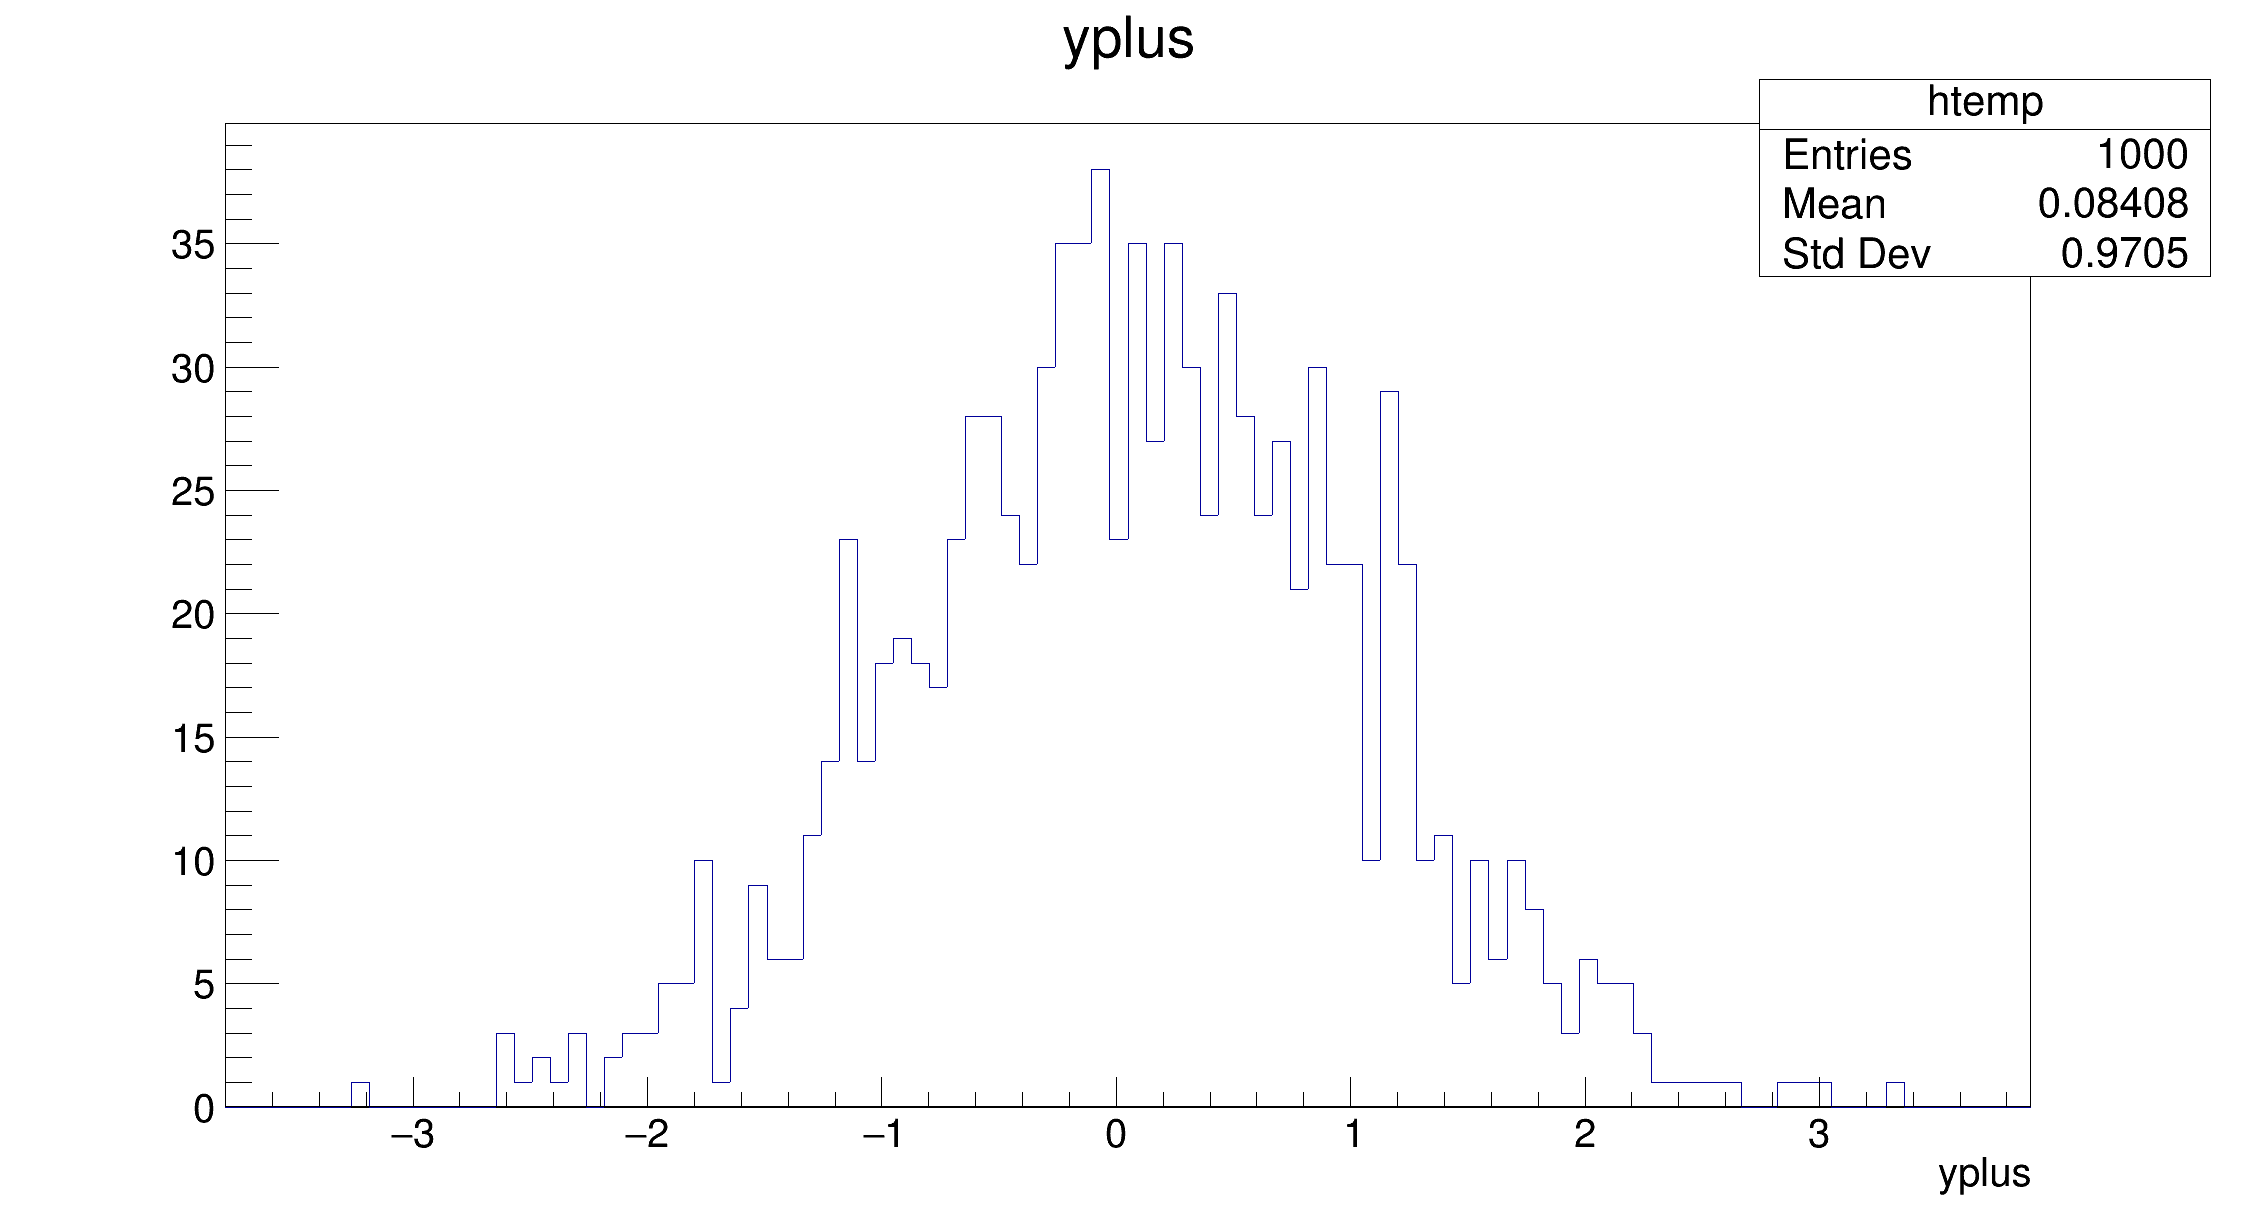
\includegraphics[width = 1.0\textwidth]{yplus1K1K.png}
      \caption{$y_+$ pull}
    \end{subfigure}%
    \begin{subfigure}{0.5\textwidth}
      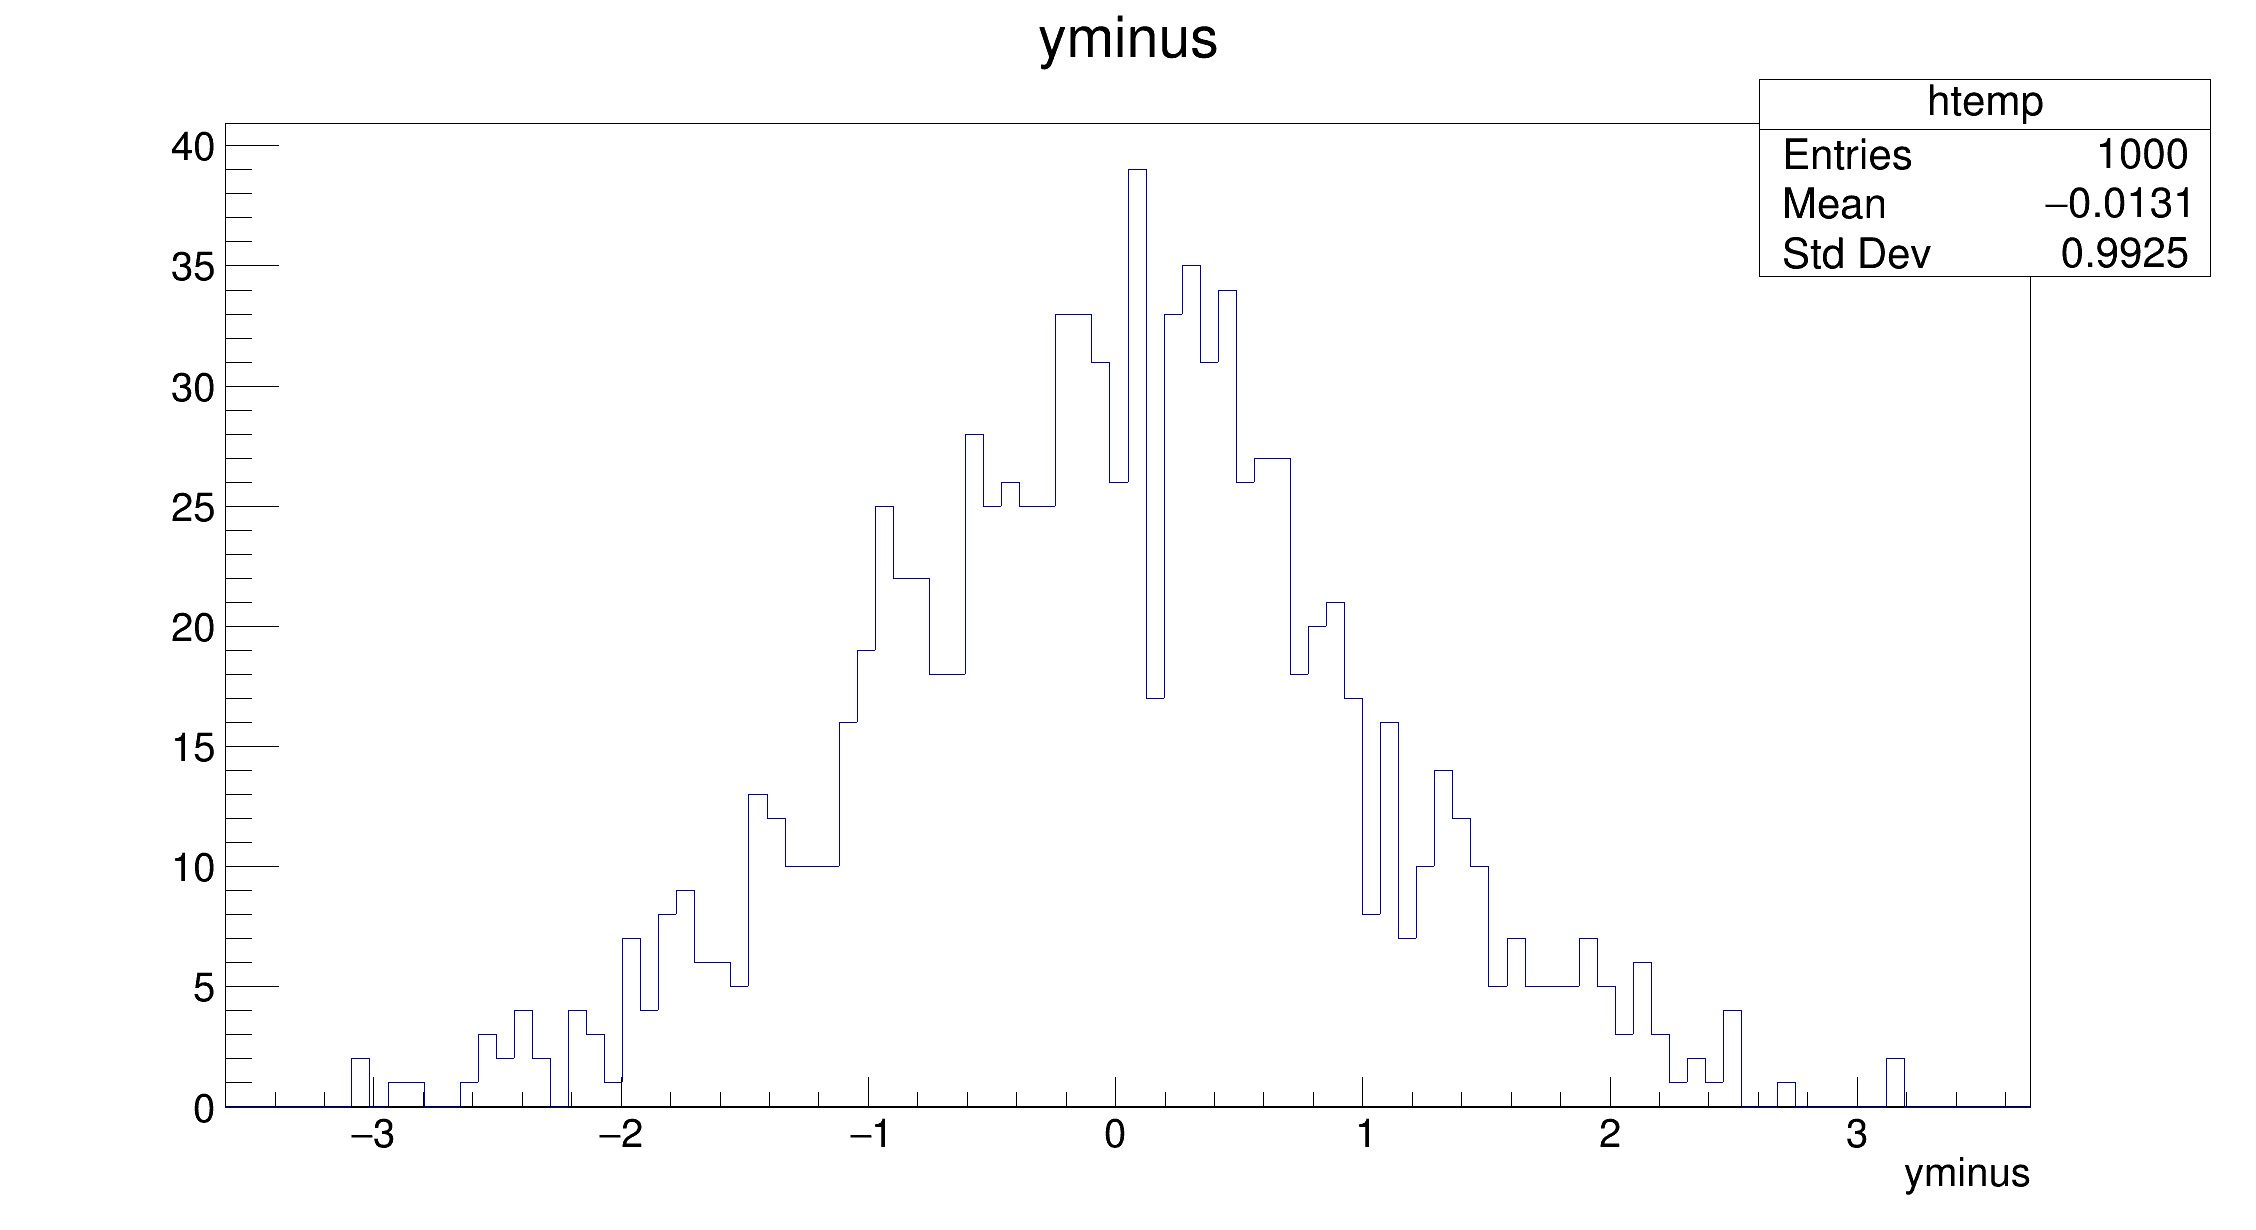
\includegraphics[width = 1.0\textwidth]{yminus1K1K.png}
      \caption{$y_-$ pull}
    \end{subfigure}
  \end{figure}
\end{frame}

\begin{frame}{Pull study with $\SI{2e4}{}$ events}
  \begin{figure}
    \centering
    \vspace{-0.2cm}
    \begin{subfigure}{0.5\textwidth}
      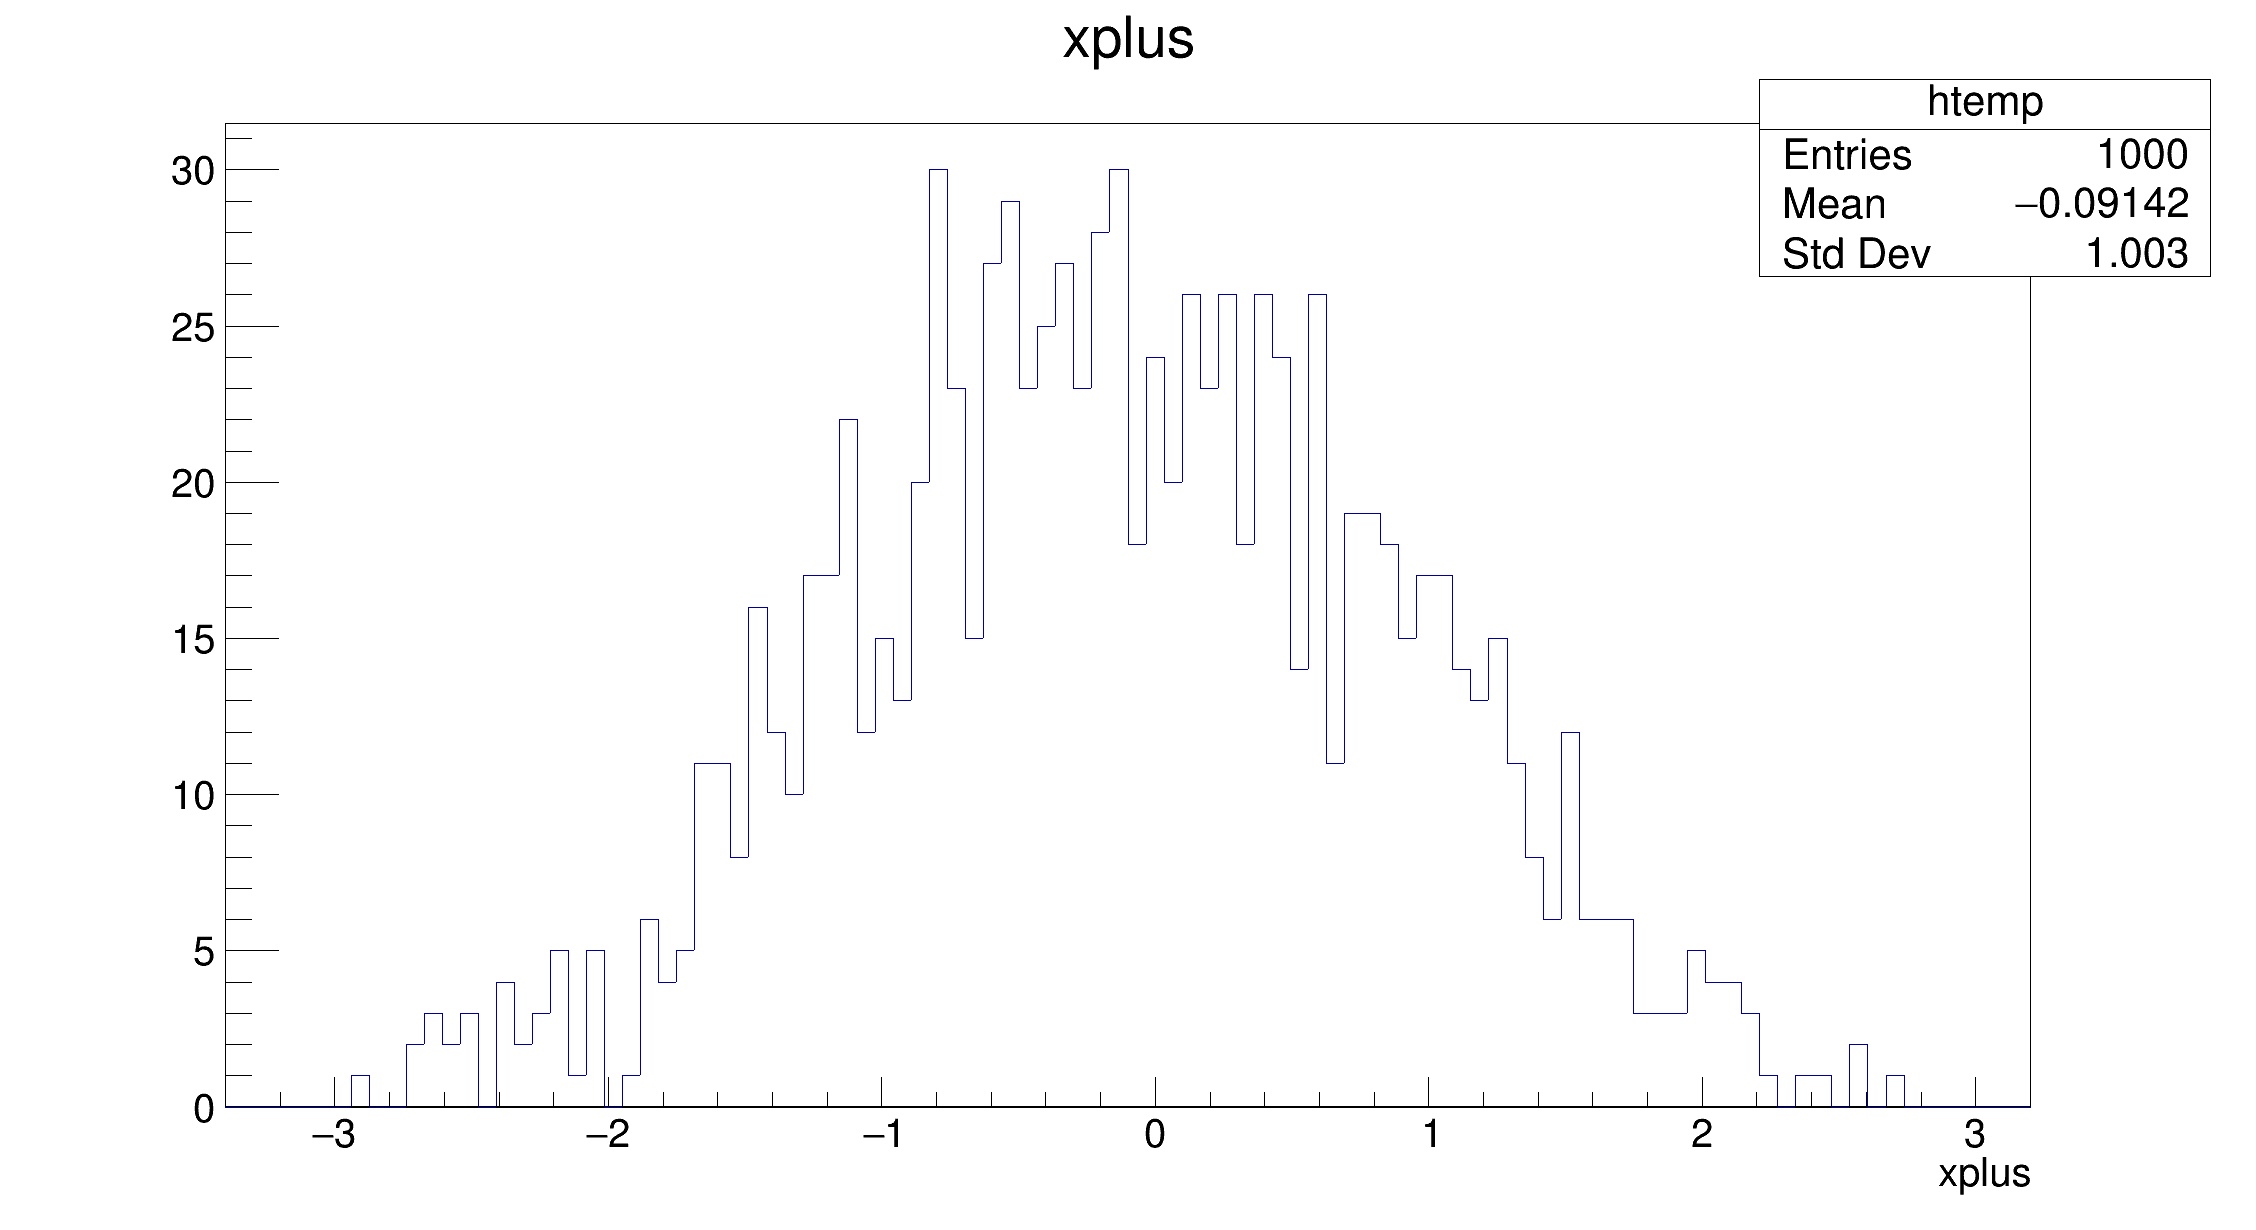
\includegraphics[width = 1.0\textwidth]{xplus10K1K.png}
      \caption{$x_+$ pull}
    \end{subfigure}%
    \begin{subfigure}{0.5\textwidth}
      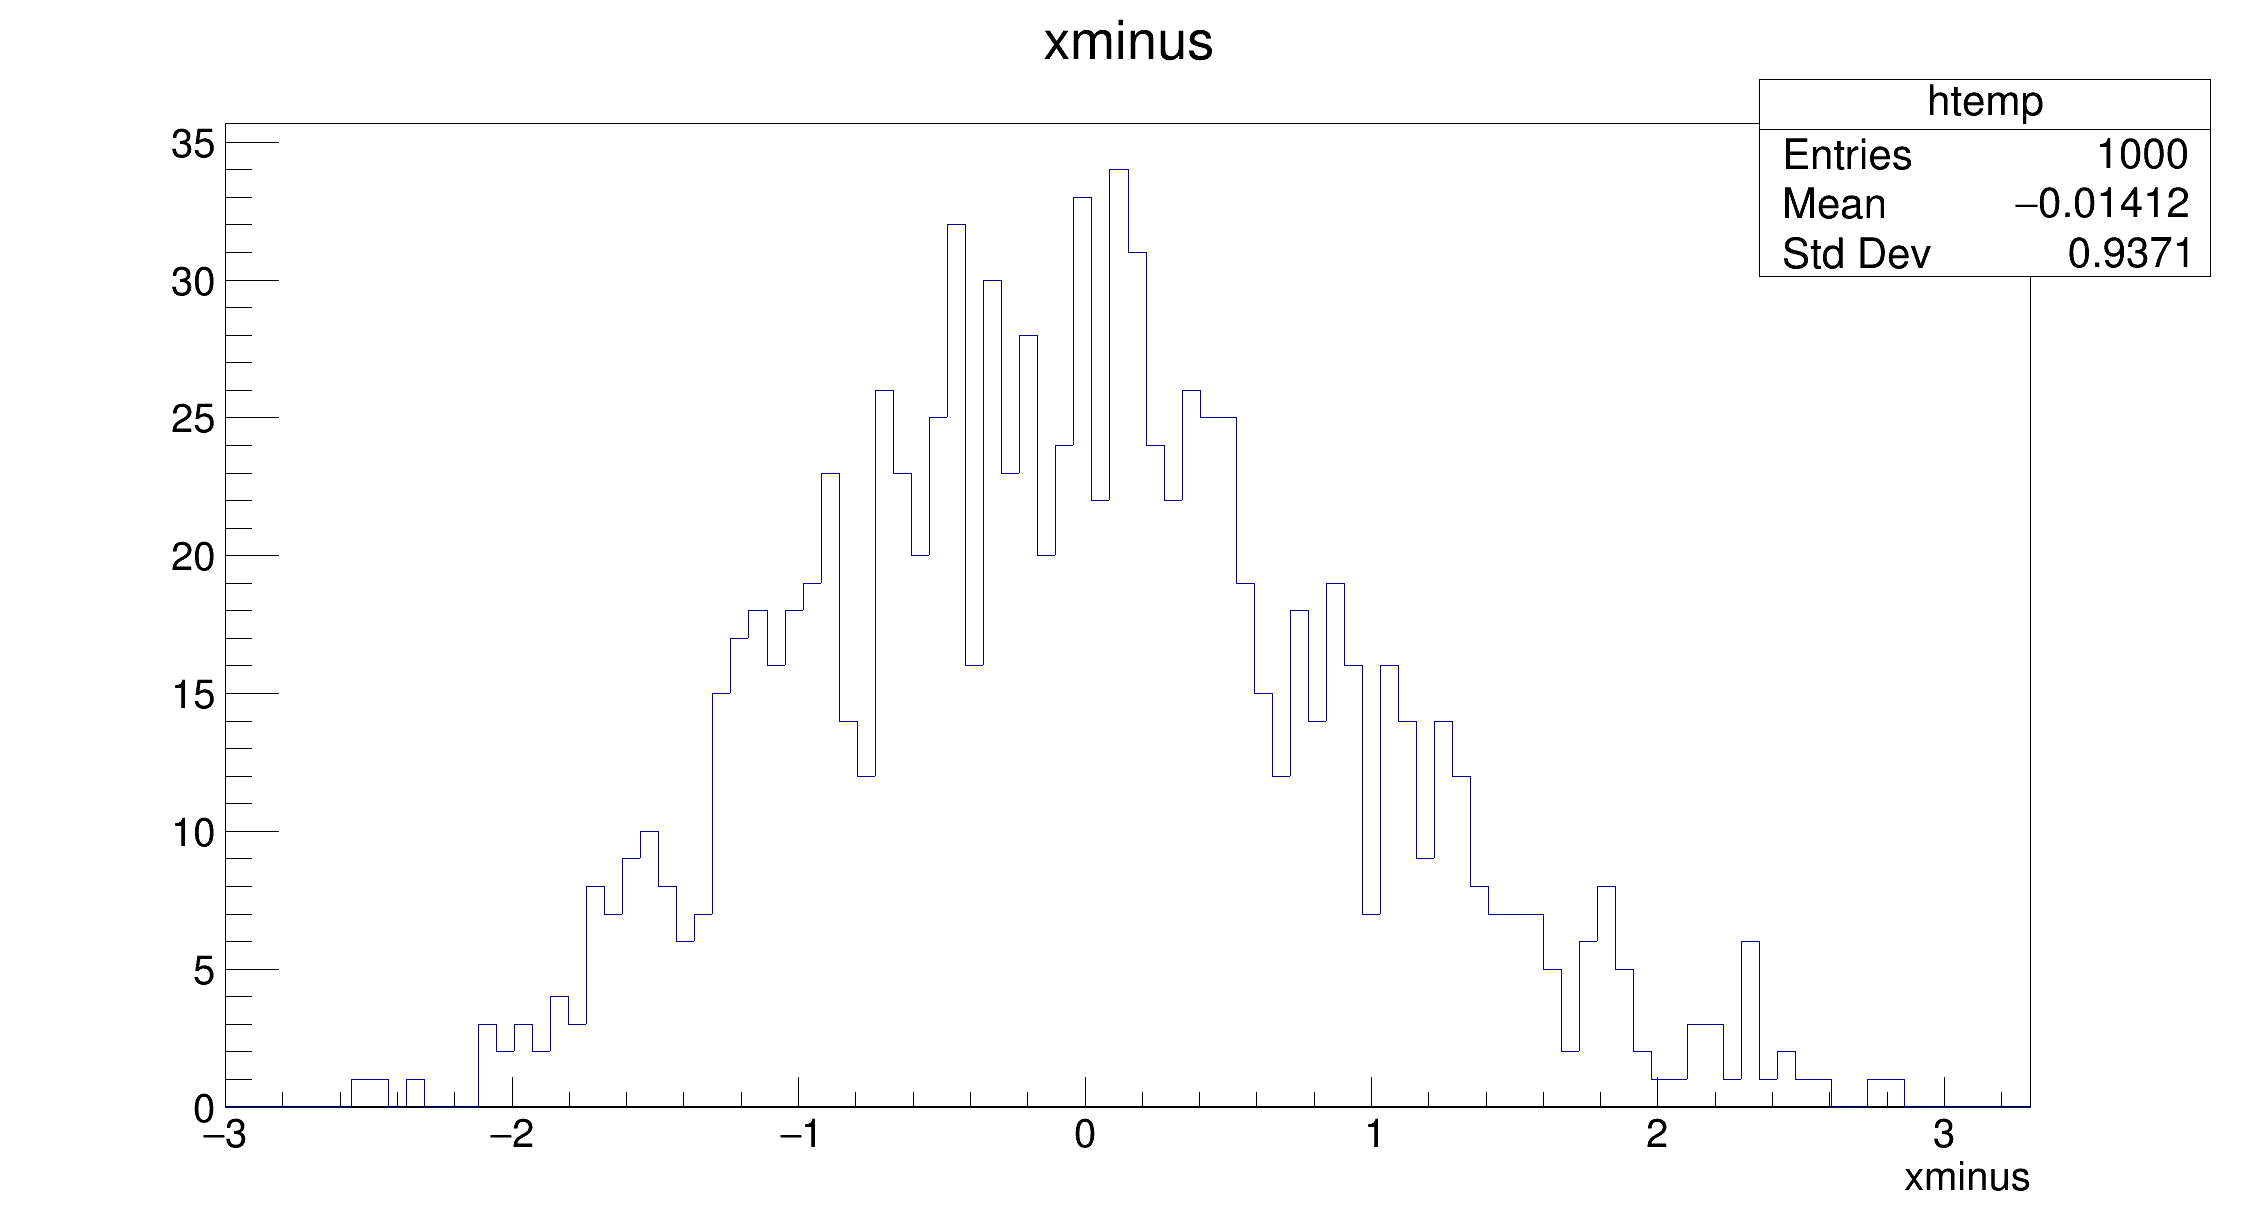
\includegraphics[width = 1.0\textwidth]{xminus10K1K.png}
      \caption{$x_-$ pull}
    \end{subfigure}
    \begin{subfigure}{0.5\textwidth}
      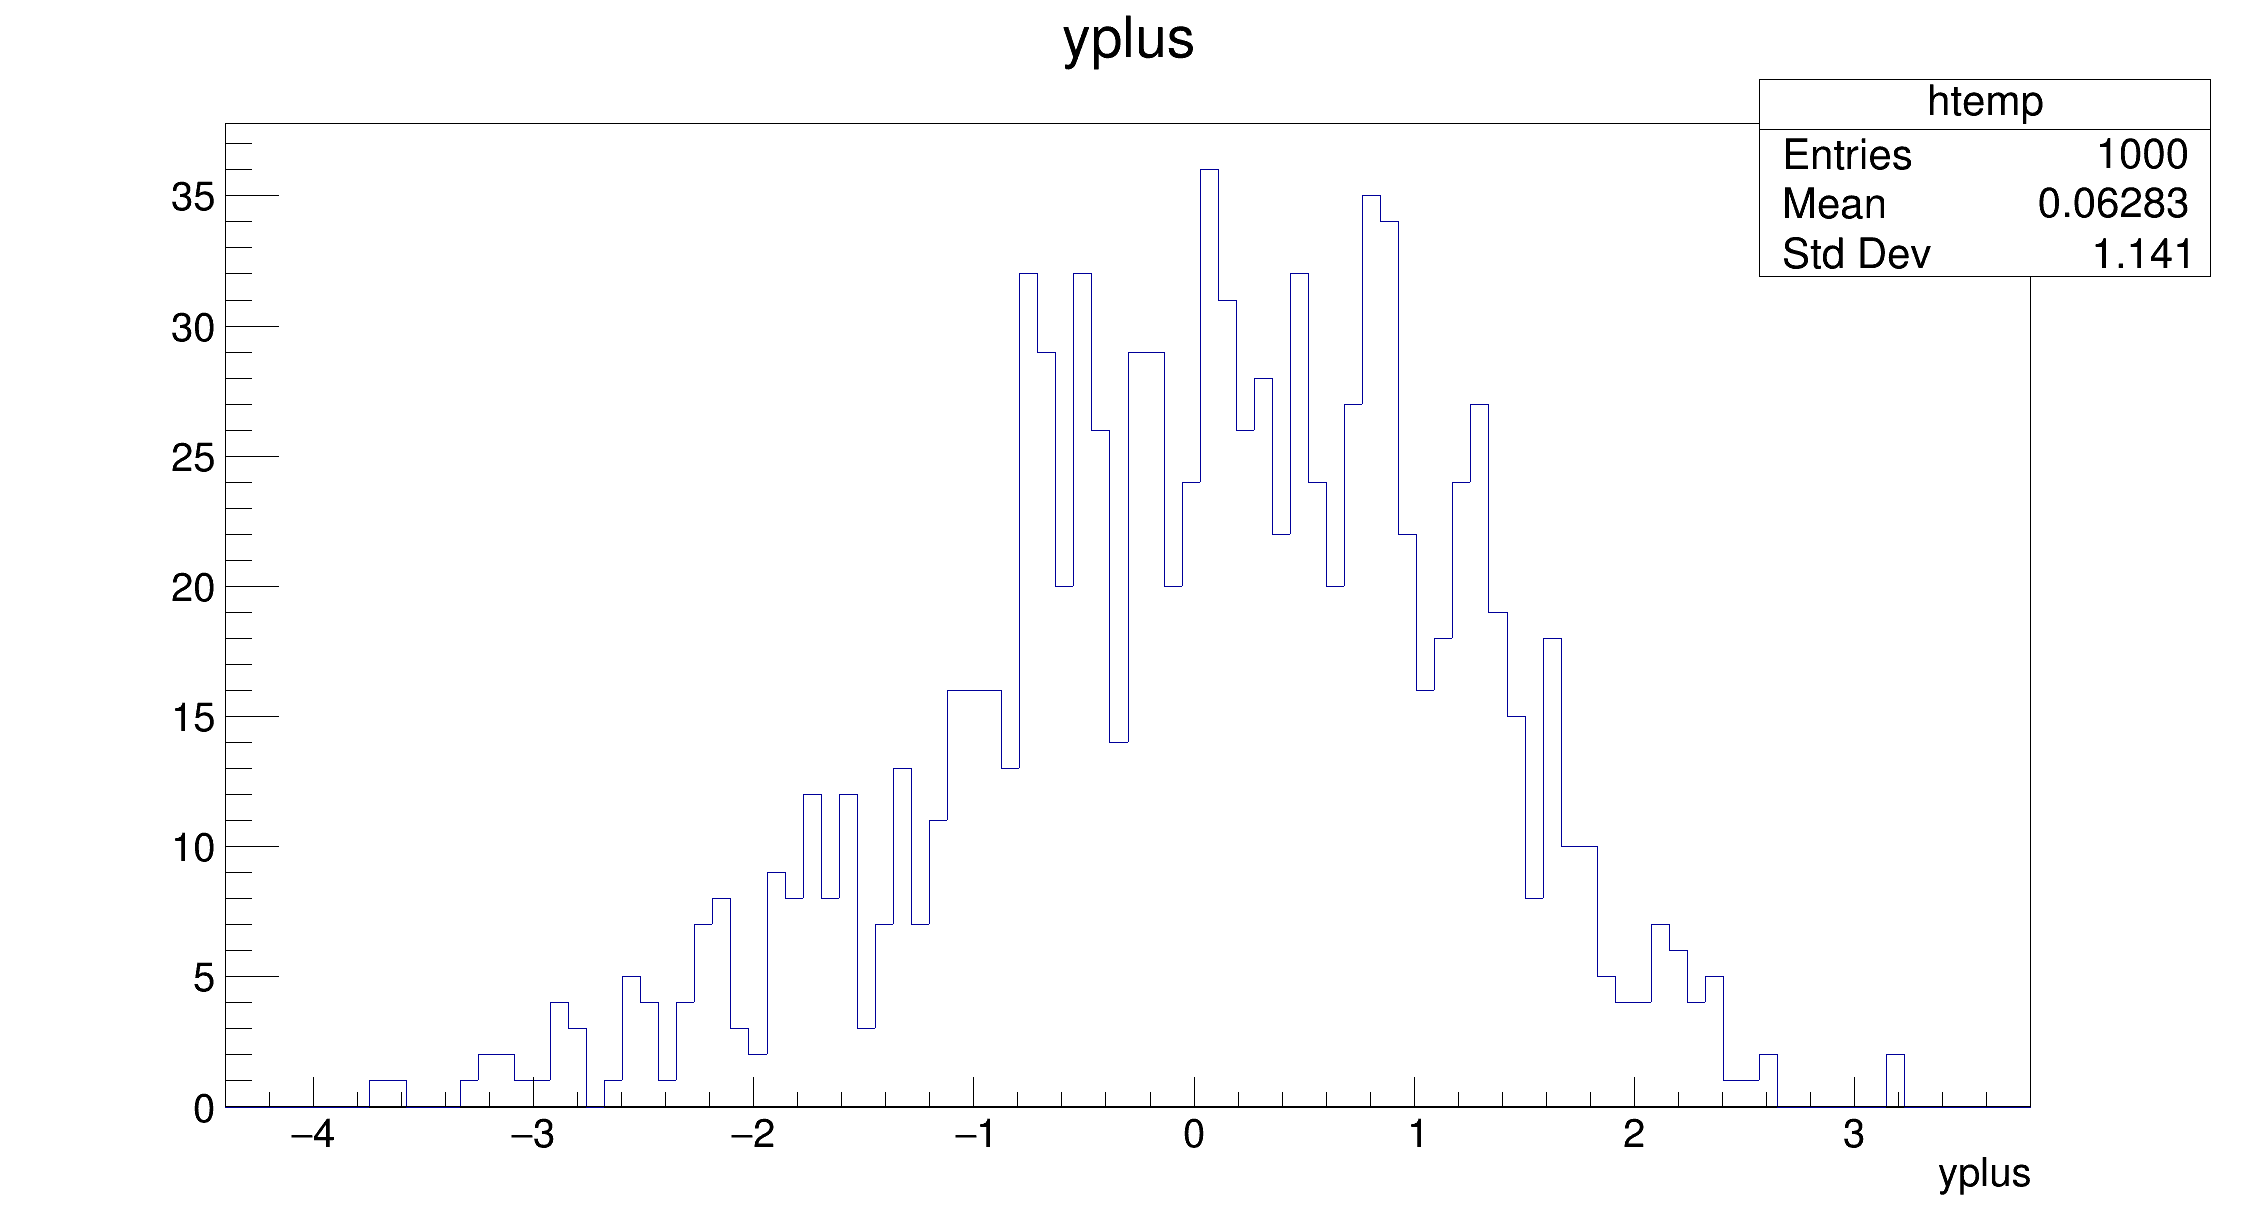
\includegraphics[width = 1.0\textwidth]{yplus10K1K.png}
      \caption{$y_+$ pull}
    \end{subfigure}%
    \begin{subfigure}{0.5\textwidth}
      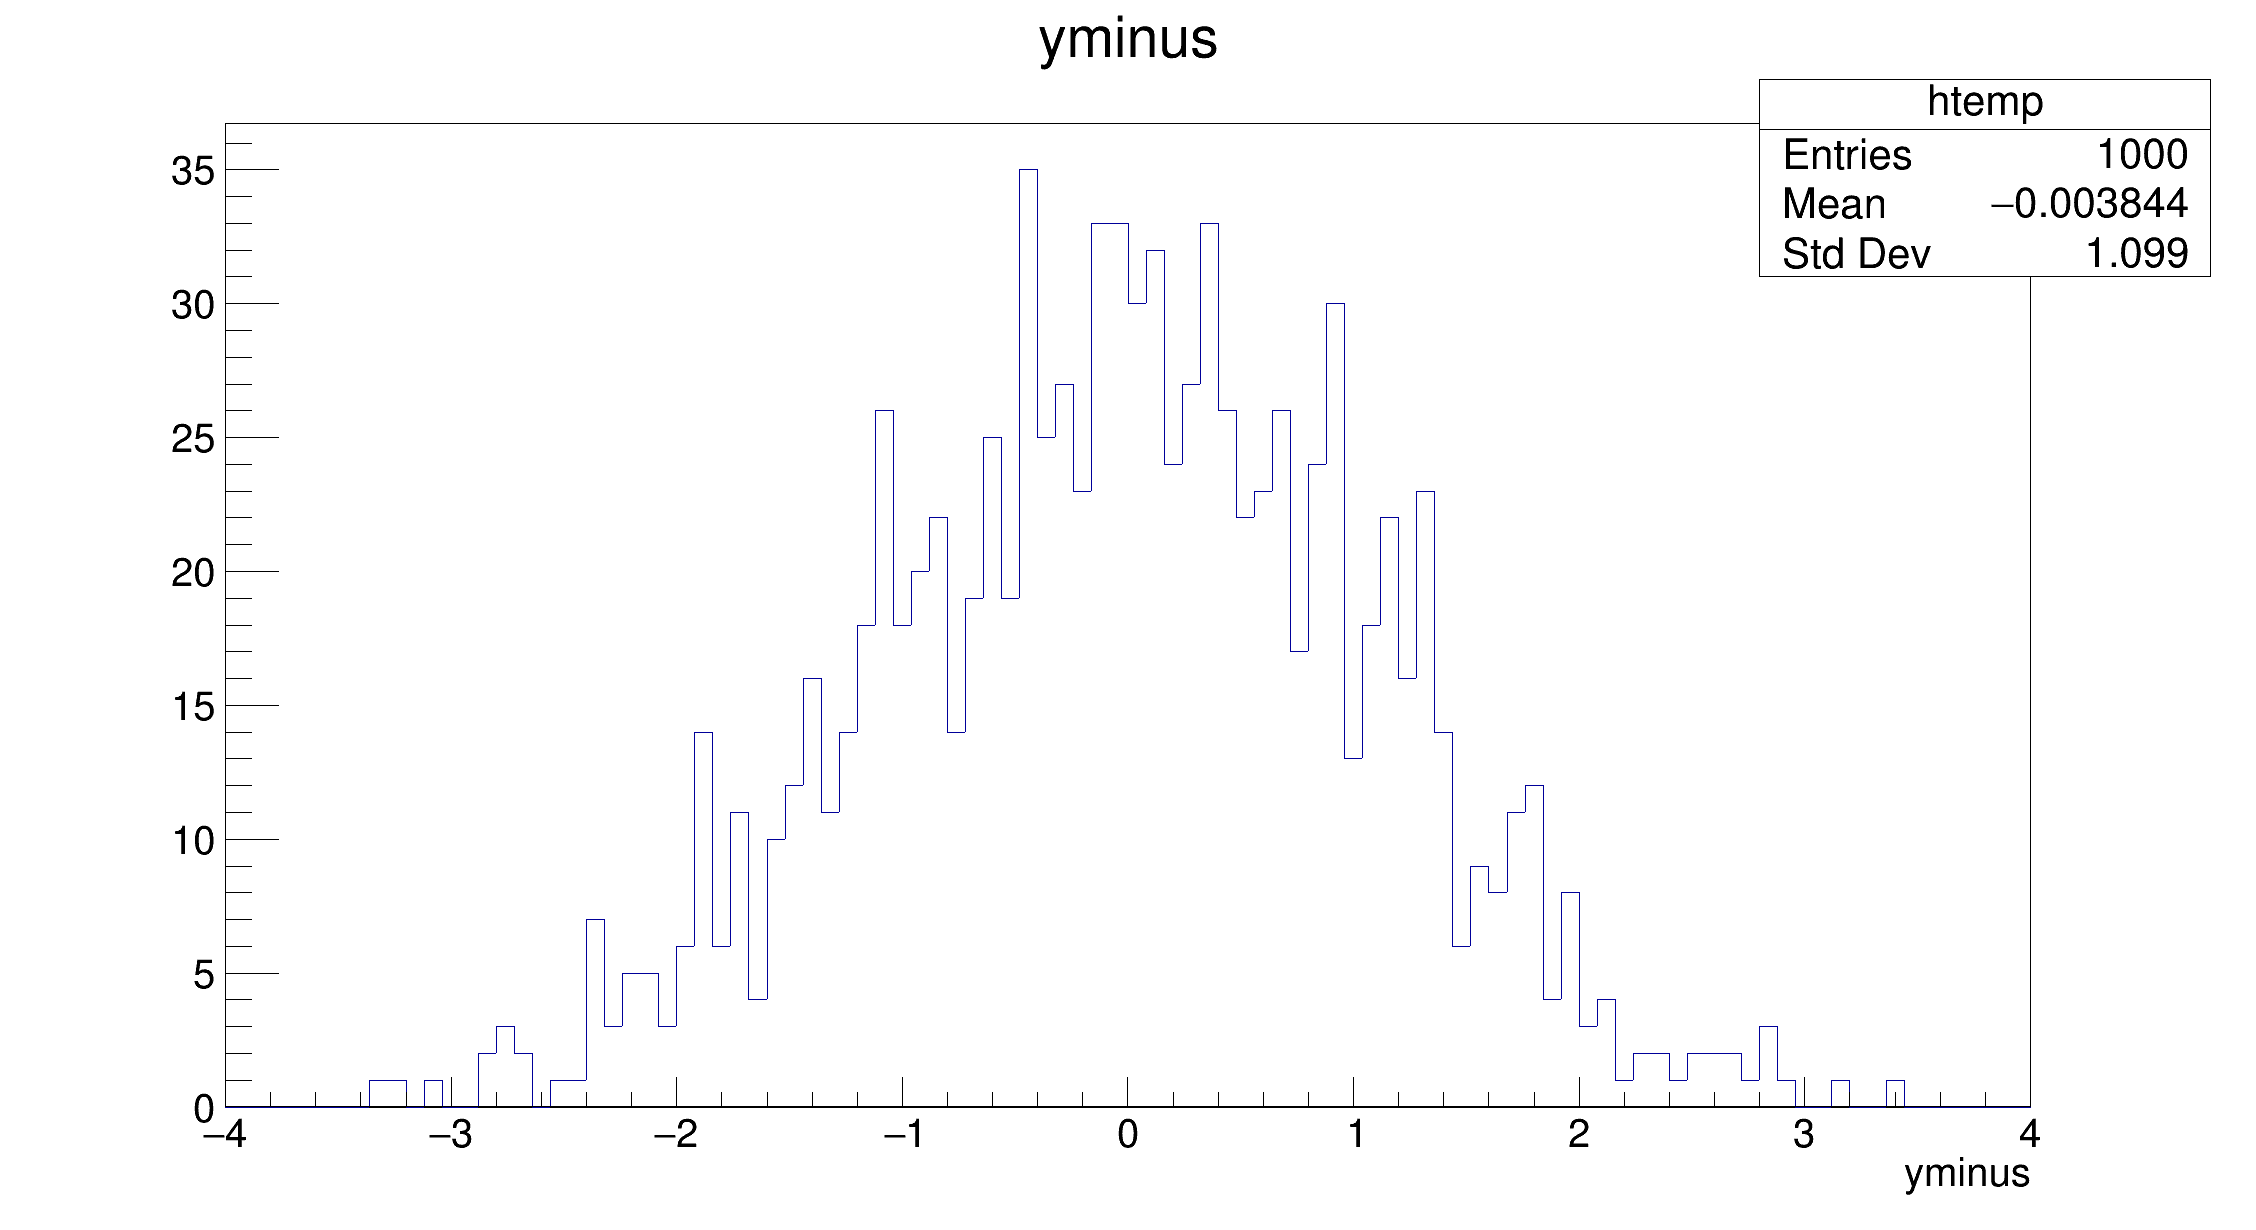
\includegraphics[width = 1.0\textwidth]{yminus10K1K.png}
      \caption{$y_-$ pull}
    \end{subfigure}
  \end{figure}
\end{frame}

\begin{frame}{Parameterisation of phase space}
  \begin{itemize}
    \item{$4$-body phase space is $5$-dimensional}
    \item{Convenient to choose rectangular coordinates}
  \end{itemize}
  \begin{block}{Phase space parameterisation}
    \begin{align*}
      x_1 =& m(K^+\pi^+) + \alpha \\
      x_2 =& m(K^-\pi^-) + \alpha, \quad \alpha = \text{min}\big(m(K^+\pi^+), m(K^-\pi^-)\big) \\
      x_3 =& \cos(\theta_+), \quad \text{(Helicity angles)} \\
      x_4 =& \cos(\theta_-) \\
      x_5 =& \phi \\
    \end{align*}
  \end{block}
  \begin{itemize}
    \item{Define binning scheme in terms of these coordinates}
    \item{Ideally have a constant strong phase difference in each bin}
    \item{Determine binning scheme based on amplitude model, but final fit is model independent}
  \end{itemize}
\end{frame}

\begin{frame}{Histogram of strong phase difference}
  Strong phase difference from amplitude model:
  \begin{figure}
    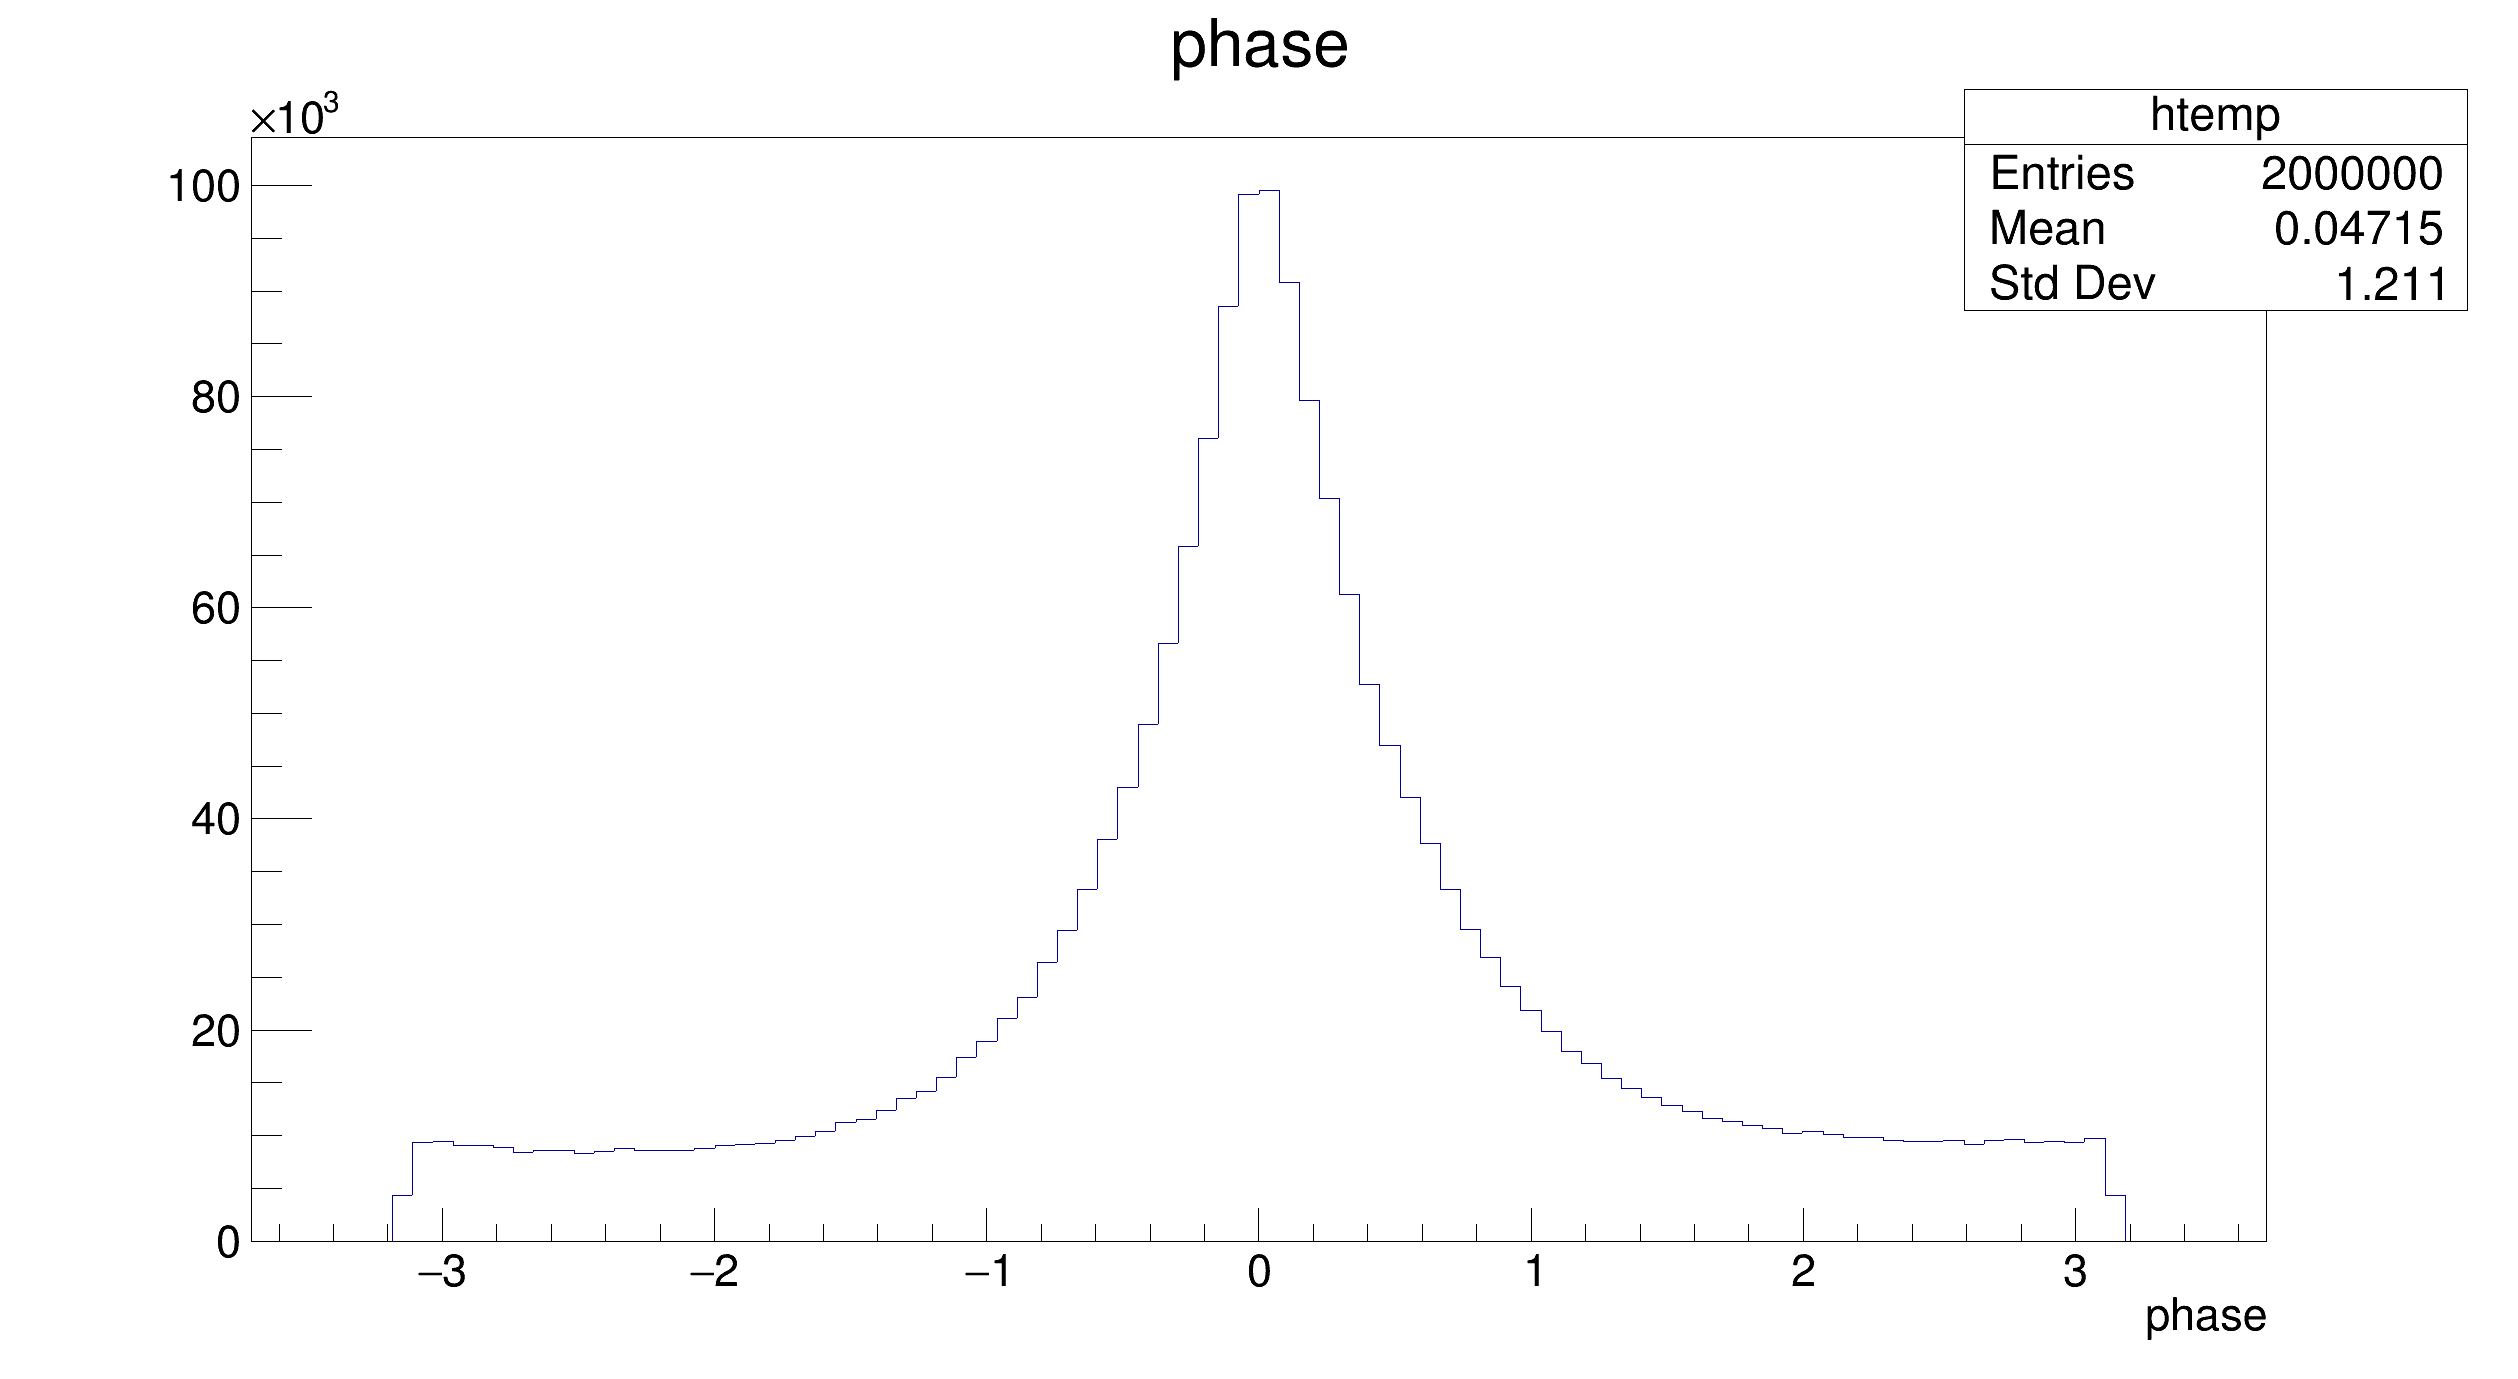
\includegraphics[width = 1\textwidth]{strongphase.png}
  \end{figure}
\end{frame}

\begin{frame}{Histogram of strong phase difference}
  Place cuts $x_3 > 0.8, x_4 > 0.8$:
  \begin{figure}
    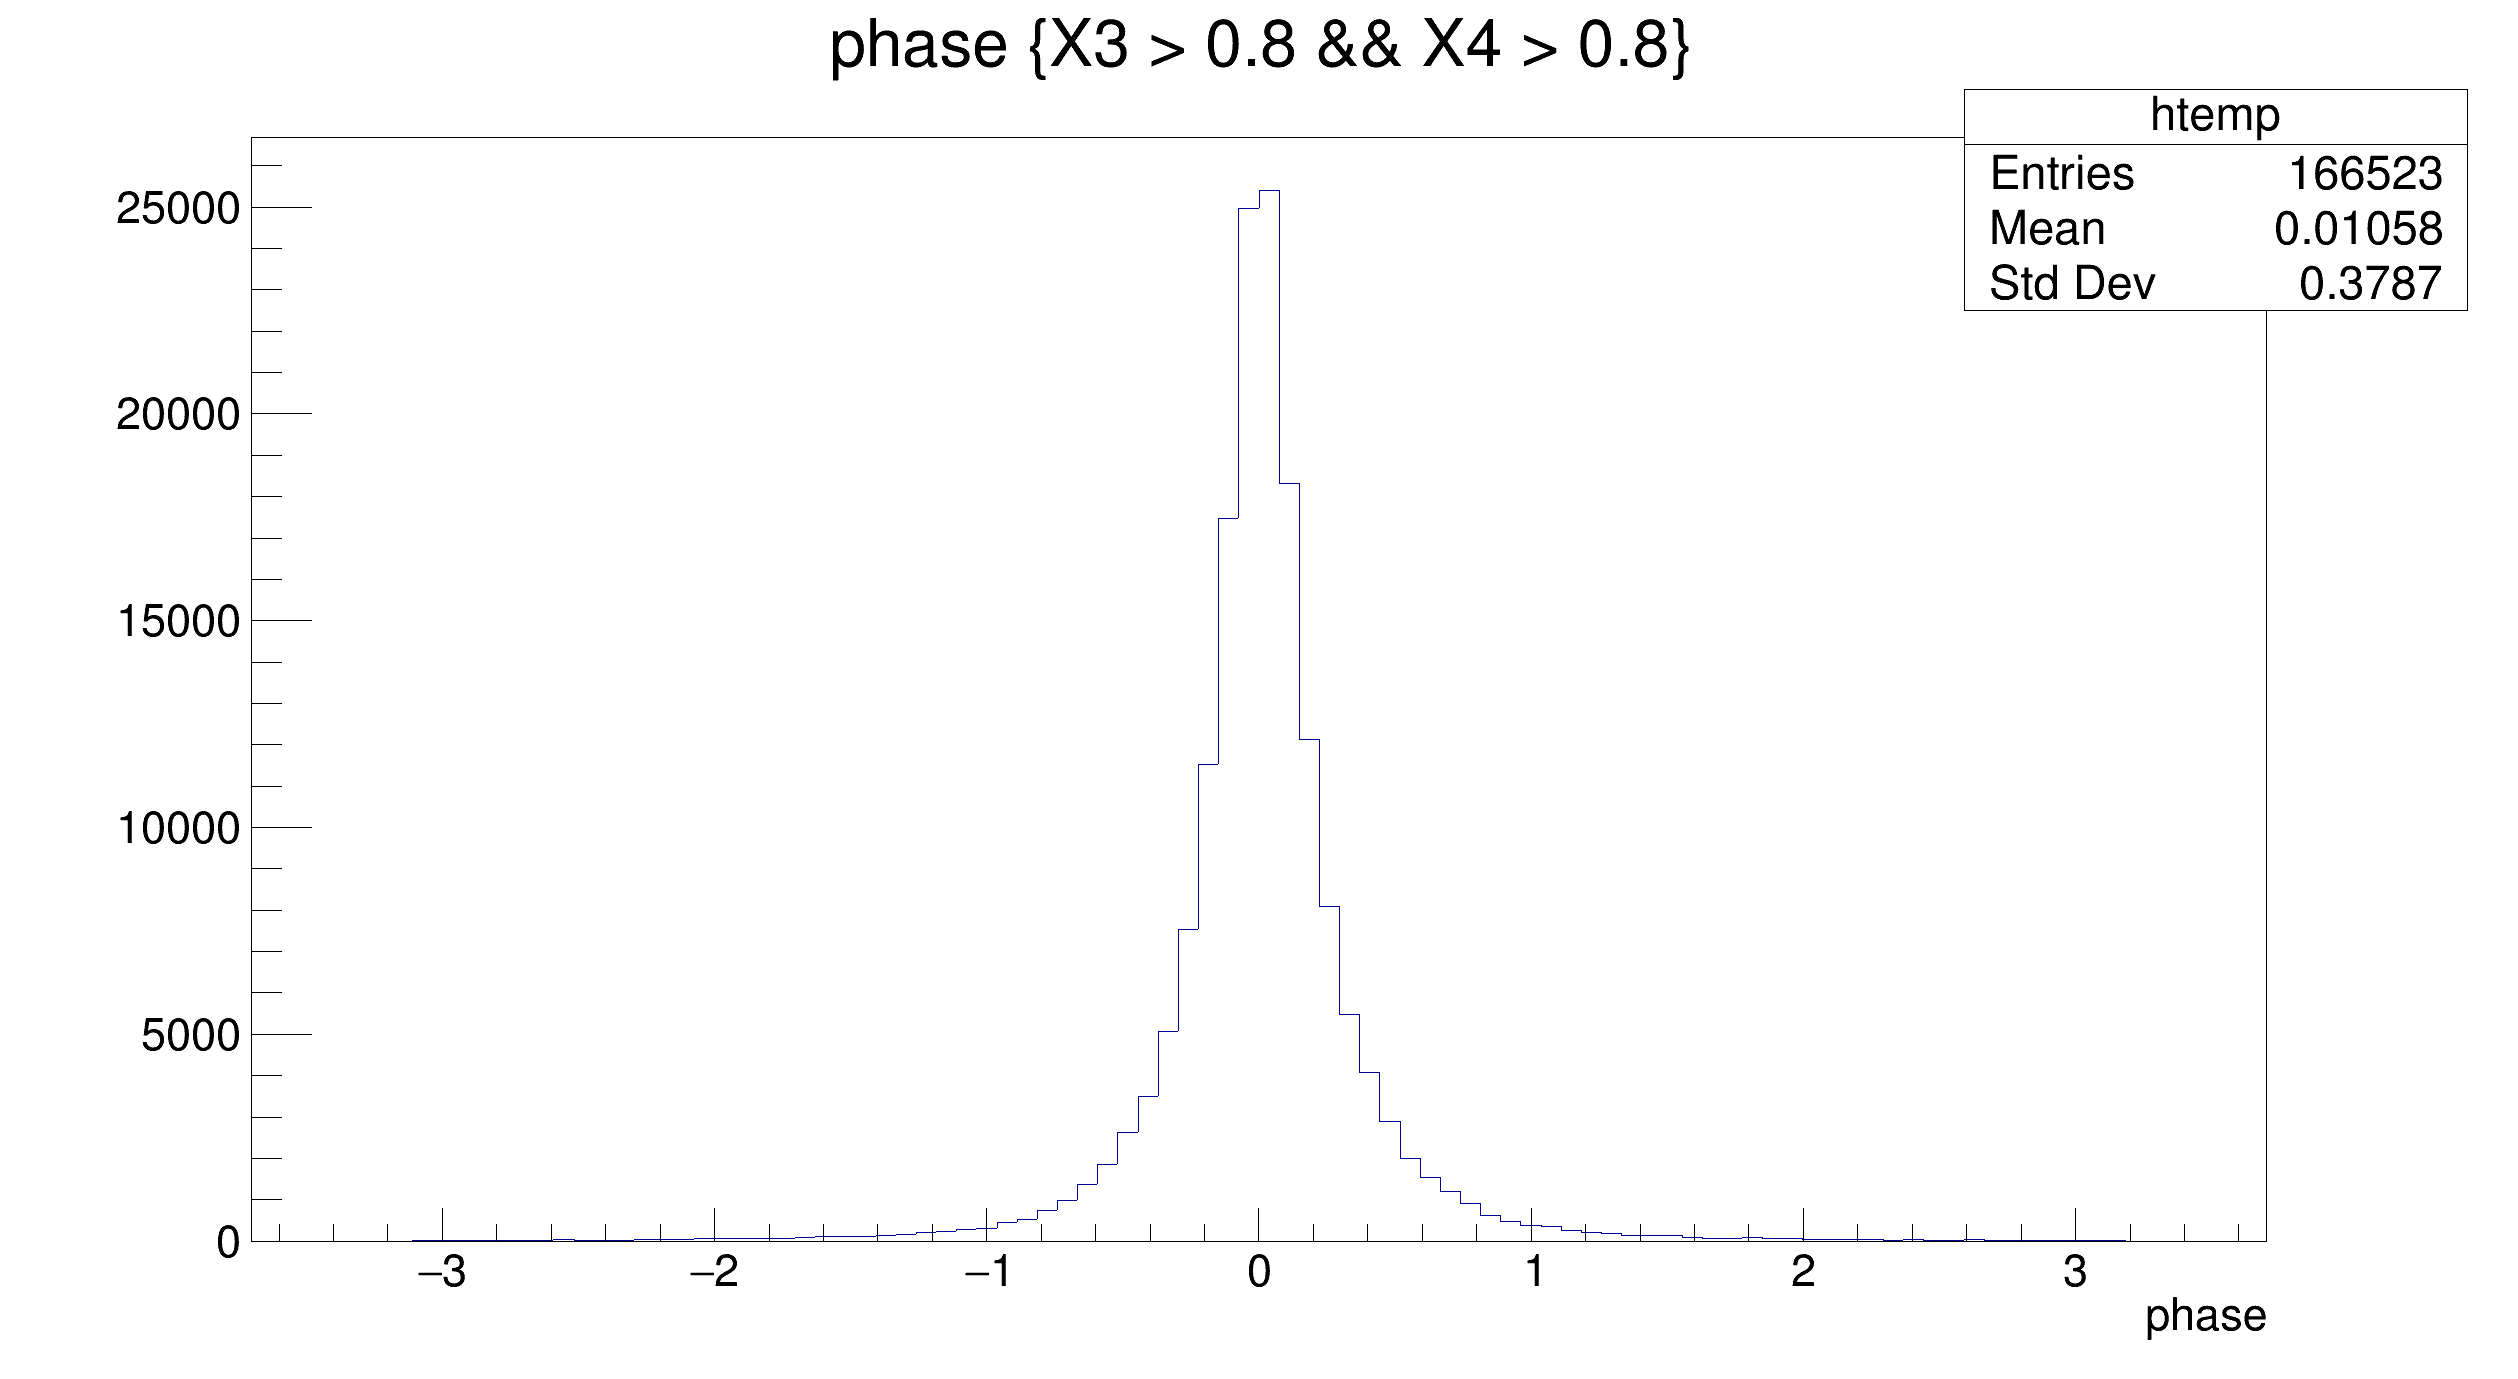
\includegraphics[width = 1\textwidth]{strongphasecut.png}
  \end{figure}
\end{frame}

\begin{frame}{Summary and next steps}
  Summary:
  \begin{itemize}
    \item{Model independent determination of $\gamma$ from $B^\pm\to(K^+K^-\pi^+\pi^-)_DK^\pm$ decay}
    \item{External input from BES III}
    \item{Precision from unbinned fit with $\SI{2e3}{}$ events: $\sigma(\gamma)\approx\SI{11}{\degree}$}
    \item{Binned fit in $5$ dimensions, need to understand phase space}
  \end{itemize}
  Next steps:
  \begin{itemize}
    \item{Finish mapping out phase space}
    \item{Decide on a suitable binning scheme}
    \item{Look at data from BES III}
    \item{Look at LHCb data}
  \end{itemize}
\end{frame}

\end{document}
